% ----------------------------------------------------------------------------------------------------
% V.5.3 - Fully Harmonized, Syntax-Corrected & Mathematically Verified
% ----------------------------------------------------------------------------------------------------

\PassOptionsToPackage{hypertexnames=false}{hyperref}
\PassOptionsToPackage{bottom=1in}{geometry}
\documentclass[sn-basic]{sn-jnl}% Basic Springer Nature Reference Style

%% Standard Packages
\usepackage{caption}
\usepackage{subcaption}
\usepackage{tikz}
\usetikzlibrary{positioning, fit, arrows.meta}
\usepackage{graphicx} % Required for \resizebox
\usepackage{pgfplots}
\pgfplotsset{compat=1.18}
\usepackage{multirow}%
\usepackage{amsmath,amssymb,amsfonts}%
\usepackage{amsthm}%
\usepackage{mathrsfs}%
\usepackage[title]{appendix}%
\usepackage{textcomp}%
\usepackage{manyfoot}%
\usepackage{setspace}
\usepackage[table]{xcolor}
\usepackage{booktabs}
\usepackage{array}

\graphicspath{{figures/}}

% --- MACRO DEFINITION ---
\newcommand{\faintcmidrule}[1]{%
	\arrayrulecolor{black!30}%
	\cmidrule{#1}%
	\arrayrulecolor{black}%
}

\newcolumntype{L}[1]{>{\raggedright\arraybackslash}p{#1}}

\makeatletter
\def\toclevel@paragraph{3}
\def\toclevel@subparagraph{4}
\makeatother

\onehalfspacing
\renewcommand{\arraystretch}{1.5}

\begin{document}

\title[RL for PdM]{Reinforcement Learning for Predictive Maintenance: A study of Attention Mechanisms for Milling Tool Replacement}

\author[1,4]{\fnm{Rajesh} \sur{Siraskar} \sfx{(\href{https://orcid.org/0000-0003-2341-8787}{ORCID: 0000-0003-2341-8787}})}\email{rajesh.siraskar@gmail.com}
\author*[1,2]{\fnm{Satish} \sur{Kumar}}\email{satish.kumar@sitpune.edu.in}
\author[1,2]{\fnm{Shruti} \sur{Patil}}
\author[1]{\fnm{Arunkumar} \sur{Bongale}}
\author[1,2]{\fnm{Ketan} \sur{Kotecha}}
\author[3]{Ambarish Kulkarni}

\affil*[1]{\orgdiv{Symbiosis Institute of Technology}, \orgname{Symbiosis International (Deemed University)}, \orgaddress{\city{Pune}, \postcode{412115}, \state{Maharashtra}, \country{India}}}
\affil[2]{\orgdiv{Symbiosis Centre for Applied Artificial Intelligence}, \orgname{Symbiosis International (Deemed University)}, \orgaddress{\city{Pune}, \postcode{412115}, \state{Maharashtra}, \country{India}}}
\affil[3]{Swinburne University of Technology, Hawthorn VIC 3122, Australia}
\affil[4]{\orgdiv{CTO Office}, \orgname{Birlasoft Ltd.}, \orgaddress{\city{Pune}, \postcode{411057}, \state{Maharashtra}, \country{India}}}

\abstract{Predictive maintenance helps decide when a machine component should be replaced. This paper studies milling cutting-tool replacement as a Reinforcement Learning (RL) problem. The decision is asymmetric: late replacement affects quality, while early replacement wastes tool life. We test whether \textsc{REINFORCE}, a Monte-Carlo policy-gradient method, can be competitive with more advanced RL baselines when paired with attention-based feature extractors. We compare \textsc{A2C}, \textsc{DQN}, \textsc{PPO}, and \textsc{REINFORCE} with four attention mechanisms on a Gymnasium-compatible milling environment, evaluated on the public IEEE PHM~2010 dataset and an in-house `SIT' dataset.

Our results reveal a clear performance hierarchy based on algorithmic family. Without attention, \textsc{PPO} is the top performer (SIT: 0.6313, IEEE: 0.7484). With attention, \textsc{REINFORCE} achieves the highest mean score in the tested settings (SIT: 0.8646 with Nadaraya--Watson; IEEE: 0.8860 with self-attention). The focused comparison shows that \textsc{REINFORCE} is not superior to \textsc{PPO} at baseline, but the difference becomes statistically supported under attention (SIT: $p=0.0007$; IEEE: $p=0.0243$). An ablation study confirms that attention significantly improves policy-gradient methods (\textsc{REINFORCE} and \textsc{PPO}) but causes performance degradation in value-based learners like \textsc{DQN}. These findings suggest that, for this PdM task, pairing policy-gradient algorithms with attention-based feature extractors is effective, with \textsc{REINFORCE} performing strongly under the tested attention settings.}

\keywords{Predictive maintenance, Industry 4.0, Reinforcement Learning, REINFORCE, Attention mechanisms, Milling machines, AutoRL}

\maketitle

\section{Introduction}
\subsection{Background}
Predictive maintenance (PdM) tries to replace or service a component before failure, while still using useful life effectively. Modern machines generate sensor data during operation, and this data can support maintenance decisions \cite{Zonta2020, Compare2020}. In milling, the cutting tool wears gradually. Since direct wear inspection usually interrupts machining, a practical method should use signals already available during cutting.

\subsection{Problem statement}
This paper studies a direct PdM question: when should a milling cutting tool be replaced? Late replacement can lead to defective parts or tool failure. Early replacement is safer, but wastes tool life and interrupts production. Reinforcement Learning (RL) is a natural fit because the agent intelligently chooses between two actions: replace or continue.

The main research question is: Can the computationally lightweight \textsc{REINFORCE} remain competitive with more advanced RL methods such as \textsc{DQN} (Deep Q-Network), \textsc{A2C} (Advantage Actor-Critic), and \textsc{PPO} (Proximal Policy Optimization) -- for milling PdM when it is paired with attention-based feature extraction, and does attention improve over a no-attention observation baseline?

\subsection{Contributions}

This study builds on our earlier work on \textsc{REINFORCE} for PdM \cite{Siraskar2025} and on our prior use of Nadaraya--Watson attention for tool-wear prediction \cite{Siraskar2024}. We also created an automated workbench that can be useful for industrial practitioners, AutoRL, that provides a common workflow for training, evaluation, and reporting across algorithms, hyperparameters, and feature extractors, similar to those proposed by \cite{Faust2019} and \cite{Mussi2022}.

The study is also motivated by a targeted literature gap. Attention is now common in prognostics and sequence modelling, but the literature is less clear on how attention-based state representations affect RL maintenance performance in sensor-driven predictive-maintenance settings.

\textbf{Research objectives and hypotheses:}
Our research objectives are to compare RL algorithms for milling PdM, test whether \textsc{REINFORCE} is competitive, evaluate attention against no-attention baselines, use one Gymnasium-compatible environment across two schemas, and report the results through the same AutoRL workflow.

We test three research themes:
\begin{itemize}
    \item \textbf{REINFORCE:} For the given predictive maintenance task for a milling machine tool replacement -- how does the lightweight \textsc{REINFORCE} algorithm perform in comparison with more advanced algorithms such as \textsc{A2C}, \textsc{DQN}, and \textsc{PPO}. This is a continued research theme from \cite{Siraskar2025}.
	\item \textbf{Attention mechanisms:} How do attention-based feature extractors affect RL algorithm \textsc{REINFORCE} performance and improve over a matched no-attention baseline in at least some schema--mechanism settings. This is an extension of the research theme from \cite{Siraskar2024}.
	\item \textbf{Environment design extensibility:} Can the same Markov Decision Process (MDP), environment design, and reward logic be used on two different milling-machine schemas (SIT\footnote{Symbiosis Institute of Technology} and IEEE). Can it accommodate different machine set-ups and sensor schemas. We do not claim direct transfer of a \emph{trained policy} from one schema to the other.
\end{itemize}

\textbf{Contributions:}
This paper contributes:
\begin{itemize}
    \item \textbf{RL comparison:} \textsc{REINFORCE}, \textsc{A2C}, \textsc{DQN}, and \textsc{PPO} are compared on a milling tool-replacement task.
    \item \textbf{Attention ablation:} four attention-style extractors are compared with matched no-attention baselines.
    \item \textbf{Schema-aware environment:} one Gymnasium-compatible environment is used with both SIT and IEEE sensor schemas.
    \item \textbf{Industrial practitioners:} an \textbf{AutoRL} workbench that can work with raw sensor readings, auto training, auto model selection, checkpointing, and reporting all in one workflow. In addition, model selection based on simpler practitioner friendly metrics that we designed, rather than episodic rewards. 
\end{itemize}

\section{Literature Review and Technical Background}
\label{sec:lit_tech}

Modern predictive maintenance systems link sensing, analytics, and operational decision-making in cyber-physical production systems \cite{Compare2020, Zonta2020}. Prescriptive maintenance extends this by recommending actions (e.g., replace vs. continue) within the workflow \cite{Ansari2019}. 

\subsection{Attention mechanisms for predictive maintenance and RL}
Attention originated as a way to relax the fixed-length bottleneck in encoder--decoder models by letting predictions depend selectively on the most relevant parts of the input \cite{Bahdanau2014, Luong2015}. The Transformer generalized this idea through self-attention and multi-head interactions, making it possible to model long-range dependencies without recurrence \cite{Vaswani2017}. For predictive-maintenance data this is attractive because sensor channels can be cross-correlated, delayed, and regime-dependent. In sequence models, the main limitation is computational: standard self-attention scales quadratically with sequence length, which becomes problematic for long sensor histories. Efficient variants such as Linformer and Performers reduce this burden and show how attention mechanisms can be adapted when temporal structure and computational budget must both be considered \cite{Wang2020Linformer, Choromanski2020}.

Attention is already well established in prognostics without RL. Attention-based remaining-useful-life models can emphasize informative timesteps, sensor channels, or degradation signatures, often improving representation quality and diagnostic visibility \cite{Chen2020, Chen2021, Costa2023}. Our prior Nadaraya--Watson attention study belongs to this stream: it showed that lightweight relevance weighting can improve milling tool-wear prediction while keeping memory and training cost low \cite{Siraskar2024}. However, these results should not be conflated with attention-based state representation for a maintenance policy. A prognostic model may estimate health accurately, yet still require a separate decision layer to determine whether and when maintenance should occur.

The RL literature uses attention for a different purpose: selective decision-making under irrelevant features, temporal dependence, and partial observability. Early work such as the Deep Attention Recurrent Q-Network combined attention with recurrent Q-learning and showed that attention can improve policy performance and provide visual evidence of what the agent is using, although gains were task-dependent and hard attention was difficult to optimize \cite{Sorokin2015}. Later work emphasized interpretability and representation learning, showing that attention can expose policy focus or suppress background information before control decisions are made \cite{Mott2019, Wu2021}. Related studies also distinguish between attention as part of the RL agent and RL being used to optimize an attention mechanism for another task \cite{BlakemanMareschal2022, Fei2021}. Across these studies, the recurring benefits are selective representation, better temporal or spatial importance assignment, and a limited form of interpretability; the recurring risks are extra complexity, training instability, and ambiguous causal interpretation of attention weights.

The strict literature on attention plus RL for predictive maintenance remains comparatively small. TranDRL uses Transformer-based sensor encoding for remaining-useful-life estimation and then passes the resulting health representation to a deep RL maintenance policy, creating a system-level integration of attention and prescriptive decision-making \cite{Zhao2024}. More recent work moves attention closer to the policy side: Li et al. use an attention-enhanced DQN for finite-horizon maintenance optimization, while Guo and Liang use a Transformer-augmented DQN for partially observable maintenance under combined degradation and shock effects \cite{Li2025, Guo2026}. Even so, the corpus is heterogeneous and does not yet establish common benchmarks, standardized ablations, or a clear comparison across attention designs. The literature therefore suggests a specific unresolved gap: lightweight attention for PdM exists, and attention-linked RL maintenance optimization exists, but comparative evidence on attention-based state representations for sensor-driven maintenance policies is still limited. That gap motivates the present comparison of attention-style feature extractors with lightweight and deep RL baselines. Table~\ref{tab:attention_funnel_synthesis} summarizes this progression from general attention mechanisms to attention-enhanced RL for predictive maintenance.

\begin{table}[h]
\centering
\caption{From attention in general to RL with attention mechanisms for PdM.}
\label{tab:attention_funnel_synthesis}
	\begin{tabular}{L{0.18\linewidth} L{0.30\linewidth} L{0.20\linewidth} L{0.30\linewidth}}
	\toprule
	\textbf{Stage} & \textbf{Main function of attention} & \textbf{Representative research articles} & \textbf{Main limitation for the next stage}\\
	\midrule
	Attention mechanisms generally & Selectively weight inputs and model long-range dependencies & \cite{Bahdanau2014,Vaswani2017,Luong2015} & Standard self-attention can be computationally expensive for long sequences and edge devices\\
	Efficient and lightweight attention & Reduce memory and time costs while preserving useful interactions & \cite{Choromanski2020, Siraskar2024,Wang2020Linformer} & Efficient attention alone does not make maintenance decisions\\
	Attention combined with RL & Focus policy or value learning on relevant observations, history, or features & \cite{BlakemanMareschal2022,Mott2019,Sorokin2015,Wu2021} & Gains are task-dependent; interpretability and training stability remain unresolved\\
	Attention plus RL for PdM & Use attention-enhanced health representations or states to learn maintenance actions & \cite{Guo2026,Luong2015, Zhao2024} & The corpus is small, heterogeneous, and lacks lightweight edge-oriented RL attention\\
	\bottomrule
	\end{tabular}
\end{table}

\subsection{RL for predictive maintenance and lightweight baselines}
RL has been surveyed extensively in PdM, with evidence that a wide range of formulations have been explored across maintenance scheduling, inspection, and resource-constrained decision problems \cite{Siraskar2023, Ogunfowora2023, Zhang2024}. A consistent theme across these surveys is that the ``right'' RL complexity level depends on (i) the structure of the decision problem (action-space size, time horizon, and reward occurrence frequency within it) and (ii) deployment requirements (compute, memory, latency).

The literature suggests a useful two-stream picture. Many PdM and condition-based maintenance studies learn effective policies using non-deep or otherwise lightweight RL, especially when state representations are structured and action spaces are modest \cite{Adsule2020, Yousefi2020, Rasay2024, Dadash2024}. Deep RL (e.g., DQN/PPO-style methods) becomes more prominent as environments become richer and harder: higher-dimensional sensing, long-horizon tradeoffs, multi-component scheduling, or coupled resource constraints \cite{Liu2020, Chen2023, Lee2022, Ong2022-02}. Recent review work also positions \textsc{REINFORCE} as comparatively underexplored in PdM \cite{Siraskar2025}.

\paragraph{Lightweight RL for edge PdM:}
Existing research indicates that lightweight methods are often a sound engineering choice when the PdM task is structured and edge constraints are first-order requirements \cite{Compare2020, Njor2024, Pandey2023}. In embedded RL more broadly, deep RL frequently requires additional techniques such as transfer learning, pruning, compression, or distillation, to fit constrained edge devices \cite{Jang2020, Szydlo2022, Xu2022}. For heavier deep models to be suitable for edge deployment, additional compression steps (e.g., pruning or quantization) are often required \cite{Pandey2023, Jang2020, Xu2022}.

Maintenance optimization contributes to energy and emissions objectives. However, these studies rarely report \emph{algorithm-level} energy or carbon for RL training and deployment, leaving a need for more focused energy studies in this direction \cite{Banyai2021, Banyai2022, JasiulewiczKaczmarek2024}.

Although RL is often motivated through generic benchmark environments, the evidence most useful for predictive maintenance comes from studies built on maintenance-specific data, assets, and decision constraints rather than abstract control tasks \cite{Andrade2021Aircraft,Dangut2022RareFailure,Zhao2024,Siraskar2025}. Public PdM benchmarks have helped move the field forward, but they still leave a gap to deployment because they cannot fully capture plant-specific degradation, sensing, and maintenance logic. By contrast, studies grounded in operational aircraft logs, fleet maintenance records, or physical manufacturing systems provide a stronger evidence tier for industrial relevance \cite{Andrade2021Aircraft,Dangut2022RareFailure,Chen2024DigitalTwin}. This matters even more for attention-based models, whose value depends on exploiting domain-specific temporal and cross-sensor structure \cite{Zhao2024}. In that sense, newly collected real machine data is a substantive contribution to PdM RL research rather than a mere implementation detail.

Vanilla \textsc{REINFORCE} is a comparatively lightweight policy-gradient method because it updates the policy directly from Monte Carlo returns and does not require a separately parameterized critic network; this reduces architectural overhead relative to actor--critic methods \cite{Williams1992,Sutton1999,Sutton2001}. However, ``lightweight'' here refers to algorithmic structure, rather than guaranteed lower wall-clock training time, energy use, or carbon emissions: Monte Carlo policy-gradient estimates can have high variance, so stable learning may still require more episodes or updates \cite{Greensmith2005}. 

For Industry 4.0 aligned intelligent predictive maintenance systems, edge deployment improves latency and resilience but imposes feasibility constraints on compute, memory, and system integration, which can limit adoption of complex ML/RL pipelines \cite{Njor2024, Pandey2023}. Research in the direction of lightweight ML or RL models helps in forwarding Industry 4.0 and 5.0 initiatives.

In our earlier PdM work, \textsc{REINFORCE} was also characterized as computationally simple and lightweight, although its training time could still exceed that of more sophisticated implementations \cite{Siraskar2025}. Accordingly, this article treats \textsc{REINFORCE} and attention as a focused research subject -- we study whether attention-style feature extractors can preserve REINFORCE's simplicity while improving policy quality for milling tool-replacement decisions.

\section{Materials and Methods}\label{sec:method}

\subsection{Technical background: MDP setting and RL algorithms}\label{sec:tech_background}
\paragraph{MDP notation and observation model:}
We model milling PdM as an episodic MDP $(\mathcal{S},\mathcal{A},P,R,\gamma)$, where $s \in \mathcal{S}$ is the sensor state, $a \in \mathcal{A}$ is the action, $P(s'|s,a)$ is the state transition probability, $R(s,a)$ is the reward function, and $\gamma \in [0,1]$ is the discount factor. Section~\ref{sec:env} applies this form to tool replacement.

\paragraph{RL algorithms compared:}
We compare DQN, A2C, PPO, and \textsc{REINFORCE} using the same environment and observation interface.

\subsection{Problem formulation: RL for PdM with attention} \label{sec:env}
\paragraph{Milling machines:}
Milling tools gradually wear during machining and are replaced near the end of useful life. We use $\tau = 300\,\mu\mathrm{m}$, as suggested in Section 7.4 of ISO 8688-2:1989 \citep{ISO8688-2-1989}, as the wear threshold for training, reward shaping, and evaluation.

At each decision step $t$, the agent selects $a_t\in\{0,1\}$, where $a_t=0$ means \emph{replace} and $a_t=1$ means \emph{continue}. Replacement ends the episode; continuing keeps the process running.

True wear is not available online because it requires offline inspection and measurement. The agent therefore uses in-process sensor data $\mathbf{x}_t\in\mathbb{R}^d$. Measured wear is used inside the environment only for termination and computation of rewards.

\paragraph{Attention as representation learning for sensor-driven PdM:}
Because decisions use $\mathbf{x}_t$ rather than direct wear inspection, each RL algorithm is paired with an attention-style extractor $\phi_\theta(\mathbf{x}_t)$ before the policy/value network.

\subsection{State space, action space, and reward function}
\label{sec:mdp_components}

\paragraph{State space (observation model):}
The information state is the sensor vector $\mathbf{x}_t$. The two schemas differ in sensors and channel count (Table~\ref{tab:schema_features}), but the decision meaning is fixed.

\paragraph{Dataset schemas and observation channels:}
\begin{table}[htbp]
\centering
\caption{Sensor channels used as observations by the RL environment}
\label{tab:schema_features}
	\begin{tabular}{L{0.18\linewidth} L{0.75\linewidth}}
	\toprule
	\textbf{Schema} & \textbf{Observation channels}\\
	\midrule
	SIT & Spindle vibration, table vibration, spindle sound, table sound, load-cell ($x$/$y$/$z$), spindle current\\
	IEEE & Cutting force ($x$/$y$/$z$), vibration ($x$/$y$/$z$), acoustic-emission RMS\\
	\bottomrule
	\end{tabular}
\end{table}

Observation vector for SIT schema: \texttt{Vib\_Spindle, Vib\_Table, Sound\_Spindle, Sound\_table, X\_Load\_Cell, Y\_Load\_Cell, Z\_Load\_Cell, Current}

Observation vector for IEEE schema: \texttt{force\_x, force\_y, force\_z, vibration\_x, vibration\_y, vibration\_z, acoustic\_emission\_rms}

\paragraph{Action space:}
The action space is discrete: $a_t=0$ means \emph{replace}, and $a_t=1$ means \emph{continue}.

\paragraph{Reward function and PdM asymmetry:}
PdM decisions are asymmetric. Late replacement may cause quality loss or failure; early replacement wastes useful life. The reward therefore encourages safe use, penalizes threshold violations, and rewards replacement near $\tau$.

\begin{table}[htbp]
	\centering
	\caption{Conceptual interpretation of PdM decisions with respect to flank wear \textsc{VB}}
	\label{tab:cost_view}
	\begin{tabular}{L{0.18\linewidth} L{0.32\linewidth} L{0.42\linewidth}}
		\toprule
		\textbf{Case} & \textbf{Condition} & \textbf{PdM interpretation}\\
		\midrule
		Timely replace & $a_t=0$ near \textsc{VB} $\approx\tau$ & Desired: high utilization and low violation risk.\\
		Early replace & $a_t=0$ when \textsc{VB} $\ll\tau$ & Safe but wasteful: reduces risk while discarding useful life.\\
		Late action / violation & $a_t=1$ while \textsc{VB} $>\tau$ & Worst case: elevated risk of quality loss or failure; strongly penalized.\\
		Continue safely & $a_t=1$ with \textsc{VB} $<\tau$ & Encouraged: extracts remaining useful life when safe.\\
		\bottomrule
	\end{tabular}
\end{table}

\paragraph{Reward shaping components:} The reward function uses 4 scalar quantities that allow the agent to learn an optimal tool replacement policy. Table \ref{tab:reward_components} lists $R_1$ through $R_4$ and how it shapes the policy.

\begin{table}[htbp]
	\centering
	\caption{Reward shaping components in the milling PdM environment.}
	\label{tab:reward_components}
	\begin{tabular}{L{0.20\linewidth} L{0.22\linewidth} L{0.50\linewidth}}
		\toprule
		\textbf{Component} & \textbf{Applied when} & \textbf{Effect}\\
		\midrule
		$R_1$ survival reward & Continue and safe & Encourages utilization while below threshold.\\
		$R_2$ violation penalty & Violated wear threshold and continued & Strongly discourages threshold violation.\\
		$R_3$ replacement cost & Replace action & Regularizes against replacing too early.\\
		$R_4$ near-threshold bonus & Replace near $\tau$ & Rewards timely replacement close to threshold.\\
		Stepwise bonuses & Wear ratio $\,\ge 0.7, 0.8, 0.9$ & Increases incentive as wear approaches threshold.\\
		\bottomrule
	\end{tabular}
\end{table}

\subsection{Execution implementation: learning pipeline and attention mechanisms}\label{sec:algo_desc}
\paragraph{AutoRL workflow:}\label{sec:autorl}
The AutoRL workbench allows configuring hyperparameter and setting options, such as model scoring weightages. It allows choosing which RL algorithms and attention mechanism feature extractors to try out. It can then establish the training queue, run combinations, automatically score and evaluate models. It allows viewing training history and logs and includes built-in crash recovery using model and training checkpoints, allowing long runs to resume. Figure \ref{fig:AutoRL} shows screens from the application. 

\begin{figure}[htbp!]
	\centering
	\begin{subfigure}[t]{0.8\textwidth}
		\centering
		\includegraphics[width=\linewidth]{AutoRL-1.png}
		\caption{AutoRL workbench - Main screen.}
	\end{subfigure}

	\begin{subfigure}[t]{0.8\textwidth}
		\centering
		\includegraphics[width=\linewidth]{AutoRL-2.png}
		\caption{The trained model evaluation dashboard.}
	\end{subfigure}
	\caption{The AutoRL workbench.}
	\label{fig:AutoRL}
\end{figure}

\paragraph{Simulation environment (Gymnasium-compatible milling PdM):}
We define a custom Gymnasium-compatible environment for milling-tool replacement \cite{Foundation2023}. Episode structure, actions, and reward logic are fixed; only the observation channels vary by schema.

\paragraph{Training procedure and policy architecture:}
All agents are trained using Stable-Baselines3 and a Gymnasium-compatible wrapper. Learning rate $\eta$ and discount factor $\gamma$ are swept because they are shared across algorithms and strongly affect performance \cite{Henderson2019, Shala2022AutoRL, Eimer2023}.
  
\paragraph{Attention mechanisms as feature extractors:}
\label{sec:attention}

Attention mechanisms are used as feature extractors $\phi(\mathbf{x}_t)$. They map the sensor vector into a 64-dimensional embedding for the policy/value networks. Here, ``attention'' means feature reweighting, gating, or structured fusion of the current sensor vector. Temporal context is added only through explicit positional encoding.

Accordingly, the attention modules studied here are representation blocks over the current observation rather than full sequence-attention policies over long temporal windows.

For the ablation study, the normalized sensor vector is also passed directly to the policy/value network as a no-attention baseline.

Unless otherwise stated, extractor capacity was held fixed across algorithms and schemas to keep the comparison controlled rather than separately tuning each module. In particular, all extractors output a 64-dimensional feature vector; NW uses 32 learnable prototype slots; temporal attention uses a 32-dimensional temporal code with $T_{max}=10{,}000$; and multi-head attention uses $H=8$ heads, giving $d_h=64/8=8$ per head.

\paragraph{Nadaraya--Watson attention}
Nadaraya--Watson (NW) attention works as kernel-based soft retrieval from learnable prototypes. We include it because it performed well in our earlier PdM attention work \cite{Siraskar2024}.

A standard Gaussian-kernel form is
\begin{equation}
        \mathbf{q}=W_q\mathbf{x}_t,\qquad
        \alpha_i = \frac{\exp\left(-\beta\,\lVert \mathbf{k}_i-\mathbf{q}\rVert^2\right)}{\sum_j \exp\left(-\beta\,\lVert \mathbf{k}_j-\mathbf{q}\rVert^2\right)},
        \qquad \mathbf{z}=\sum_i\alpha_i\,\mathbf{v}_i.
\end{equation}
We use learnable prototypes $\{\mathbf{k}_i,\mathbf{v}_i\}$ and bandwidth $\beta>0$. In the code, $\beta$ is enforced to be positive by optimizing $\log \beta$ and setting $\beta=\exp(\log \beta)$. The 32 prototype slots are a fixed design choice used as a lightweight surrogate memory rather than an external datastore.

\paragraph{Temporal attention}
Temporal attention (TP) adds a stage-of-life signal using sinusoidal positional encodings and a learnable temporal embedding \cite{Vaswani2017, Lim2020TFT}. It combines soft feature reweighting with a timestep encoding:
\begin{align}
	\boldsymbol{\alpha}_t &= \mathrm{softmax}\!\left(W_2\tanh\!\left(W_1\mathbf{x}_t\right)\right),
        \qquad \tilde{\mathbf{x}}_t = \mathbf{x}_t\odot\boldsymbol{\alpha}_t,\\
        \mathrm{PE}(t,2i) &= \sin\!\left(\frac{t}{{T_{max}}^{2i/d_{\mathrm{TP}}}}\right),
        \qquad \mathrm{PE}(t,2i+1)=\cos\!\left(\frac{t}{{T_{max}}^{2i/d_{\mathrm{TP}}}}\right),\\
        \mathbf{e}_t &= \mathrm{PE}(t) + \mathbf{b},
        \qquad \mathbf{z}_t = f_\theta\!\left([\tilde{\mathbf{x}}_t;\mathbf{e}_t]\right).
\end{align}
Here $t$ is the monotone counter used by the extractor, $T_{max}$ is the truncation limit, $d_{\mathrm{TP}}$ is the encoding dimension, and $f_\theta(\cdot)$ gives the feature embedding. In our implementation, we set $T_{max}=10{,}000$ for sinusoidal temporal encoding to distribute frequencies across positions, following the Transformer positional-encoding convention \cite{Vaswani2017}.

\paragraph{Multi-head attention}
Multi-head attention (MH) gates the single-timestep feature vector in parallel subspaces \cite{Vaswani2017}. The heads operate on projections of the current observation, not on a token sequence.

In our implementation,
\begin{align}
        \mathbf{Q}&=W^Q\mathbf{x}_t,\quad \mathbf{K}=W^K\mathbf{x}_t,\quad \mathbf{V}=W^V\mathbf{x}_t,\\
        \mathbf{q}_h&=\mathrm{split}_h(\mathbf{Q}),\quad \mathbf{k}_h=\mathrm{split}_h(\mathbf{K}),\quad \mathbf{v}_h=\mathrm{split}_h(\mathbf{V}),\\
        s_h&=\frac{\mathbf{q}_h^\top\mathbf{k}_h}{\sqrt{d_h}},\quad \alpha_h=\mathrm{softmax}(s)_h,\\
        \mathbf{z}&=W^O\,[\alpha_1\mathbf{v}_1;\ldots;\alpha_H\mathbf{v}_H].
\end{align}

Because there is no token axis, each head contributes one scalar compatibility score $s_h$ for the current observation, and the softmax is applied across heads. This should therefore be interpreted as parallel head-wise gating of a single sensor vector, not as canonical multi-token self-attention.

\paragraph{Self-attention}
Self-attention (SA) is applied to the current observation vector. It is therefore a gated feature block with residual connections and layer normalization, not sequence self-attention over a time window.

In our implementation,
\begin{align}
		\mathbf{x}^{(b)} &= W_{\mathrm{in}}\mathbf{x}_t^{(b)},\\
		\mathbf{q}^{(b)} &= W_Q\mathbf{x}^{(b)},\quad \mathbf{k}^{(b)}=W_K\mathbf{x}^{(b)},\quad \mathbf{v}^{(b)}=W_V\mathbf{x}^{(b)},\\
		s^{(b)} &= \frac{{\mathbf{q}^{(b)}}^\top\mathbf{k}^{(b)}}{\sqrt{d}},\quad
		\alpha^{(b)}=\frac{\exp(s^{(b)})}{\sum_{b'}\exp(s^{(b')})},\\
		\mathbf{z}_1^{(b)} &= \mathrm{LN}\!\left(\mathbf{x}^{(b)}+\alpha^{(b)}\mathbf{v}^{(b)}\right),\quad
		\mathbf{z}^{(b)}=\mathrm{LN}\!\left(\mathbf{z}_1^{(b)}+\mathrm{FFN}(\mathbf{z}_1^{(b)})\right).
\end{align}
Here the gate is a scalar weight produced from the current observation and normalized over the active batch in the implementation. The feed-forward block expands from 64 to 128 hidden units and then projects back to 64. Conceptually, this is best viewed as an implementation-specific residual gating block over the current sensor vector, rather than canonical sequence self-attention.

\subsection{Datasets and evaluation protocol} \label{sec:experiment} 

We evaluate AutoRL on two milling datasets: the public IEEE PHM~2010 dataset and an in-house SIT university testbed dataset. Both are mapped to the observation interface in Section~\ref{sec:mdp_components}.

\begin{figure}[htbp!]
	\centering
	\begin{subfigure}[t]{0.48\textwidth}
		\centering
		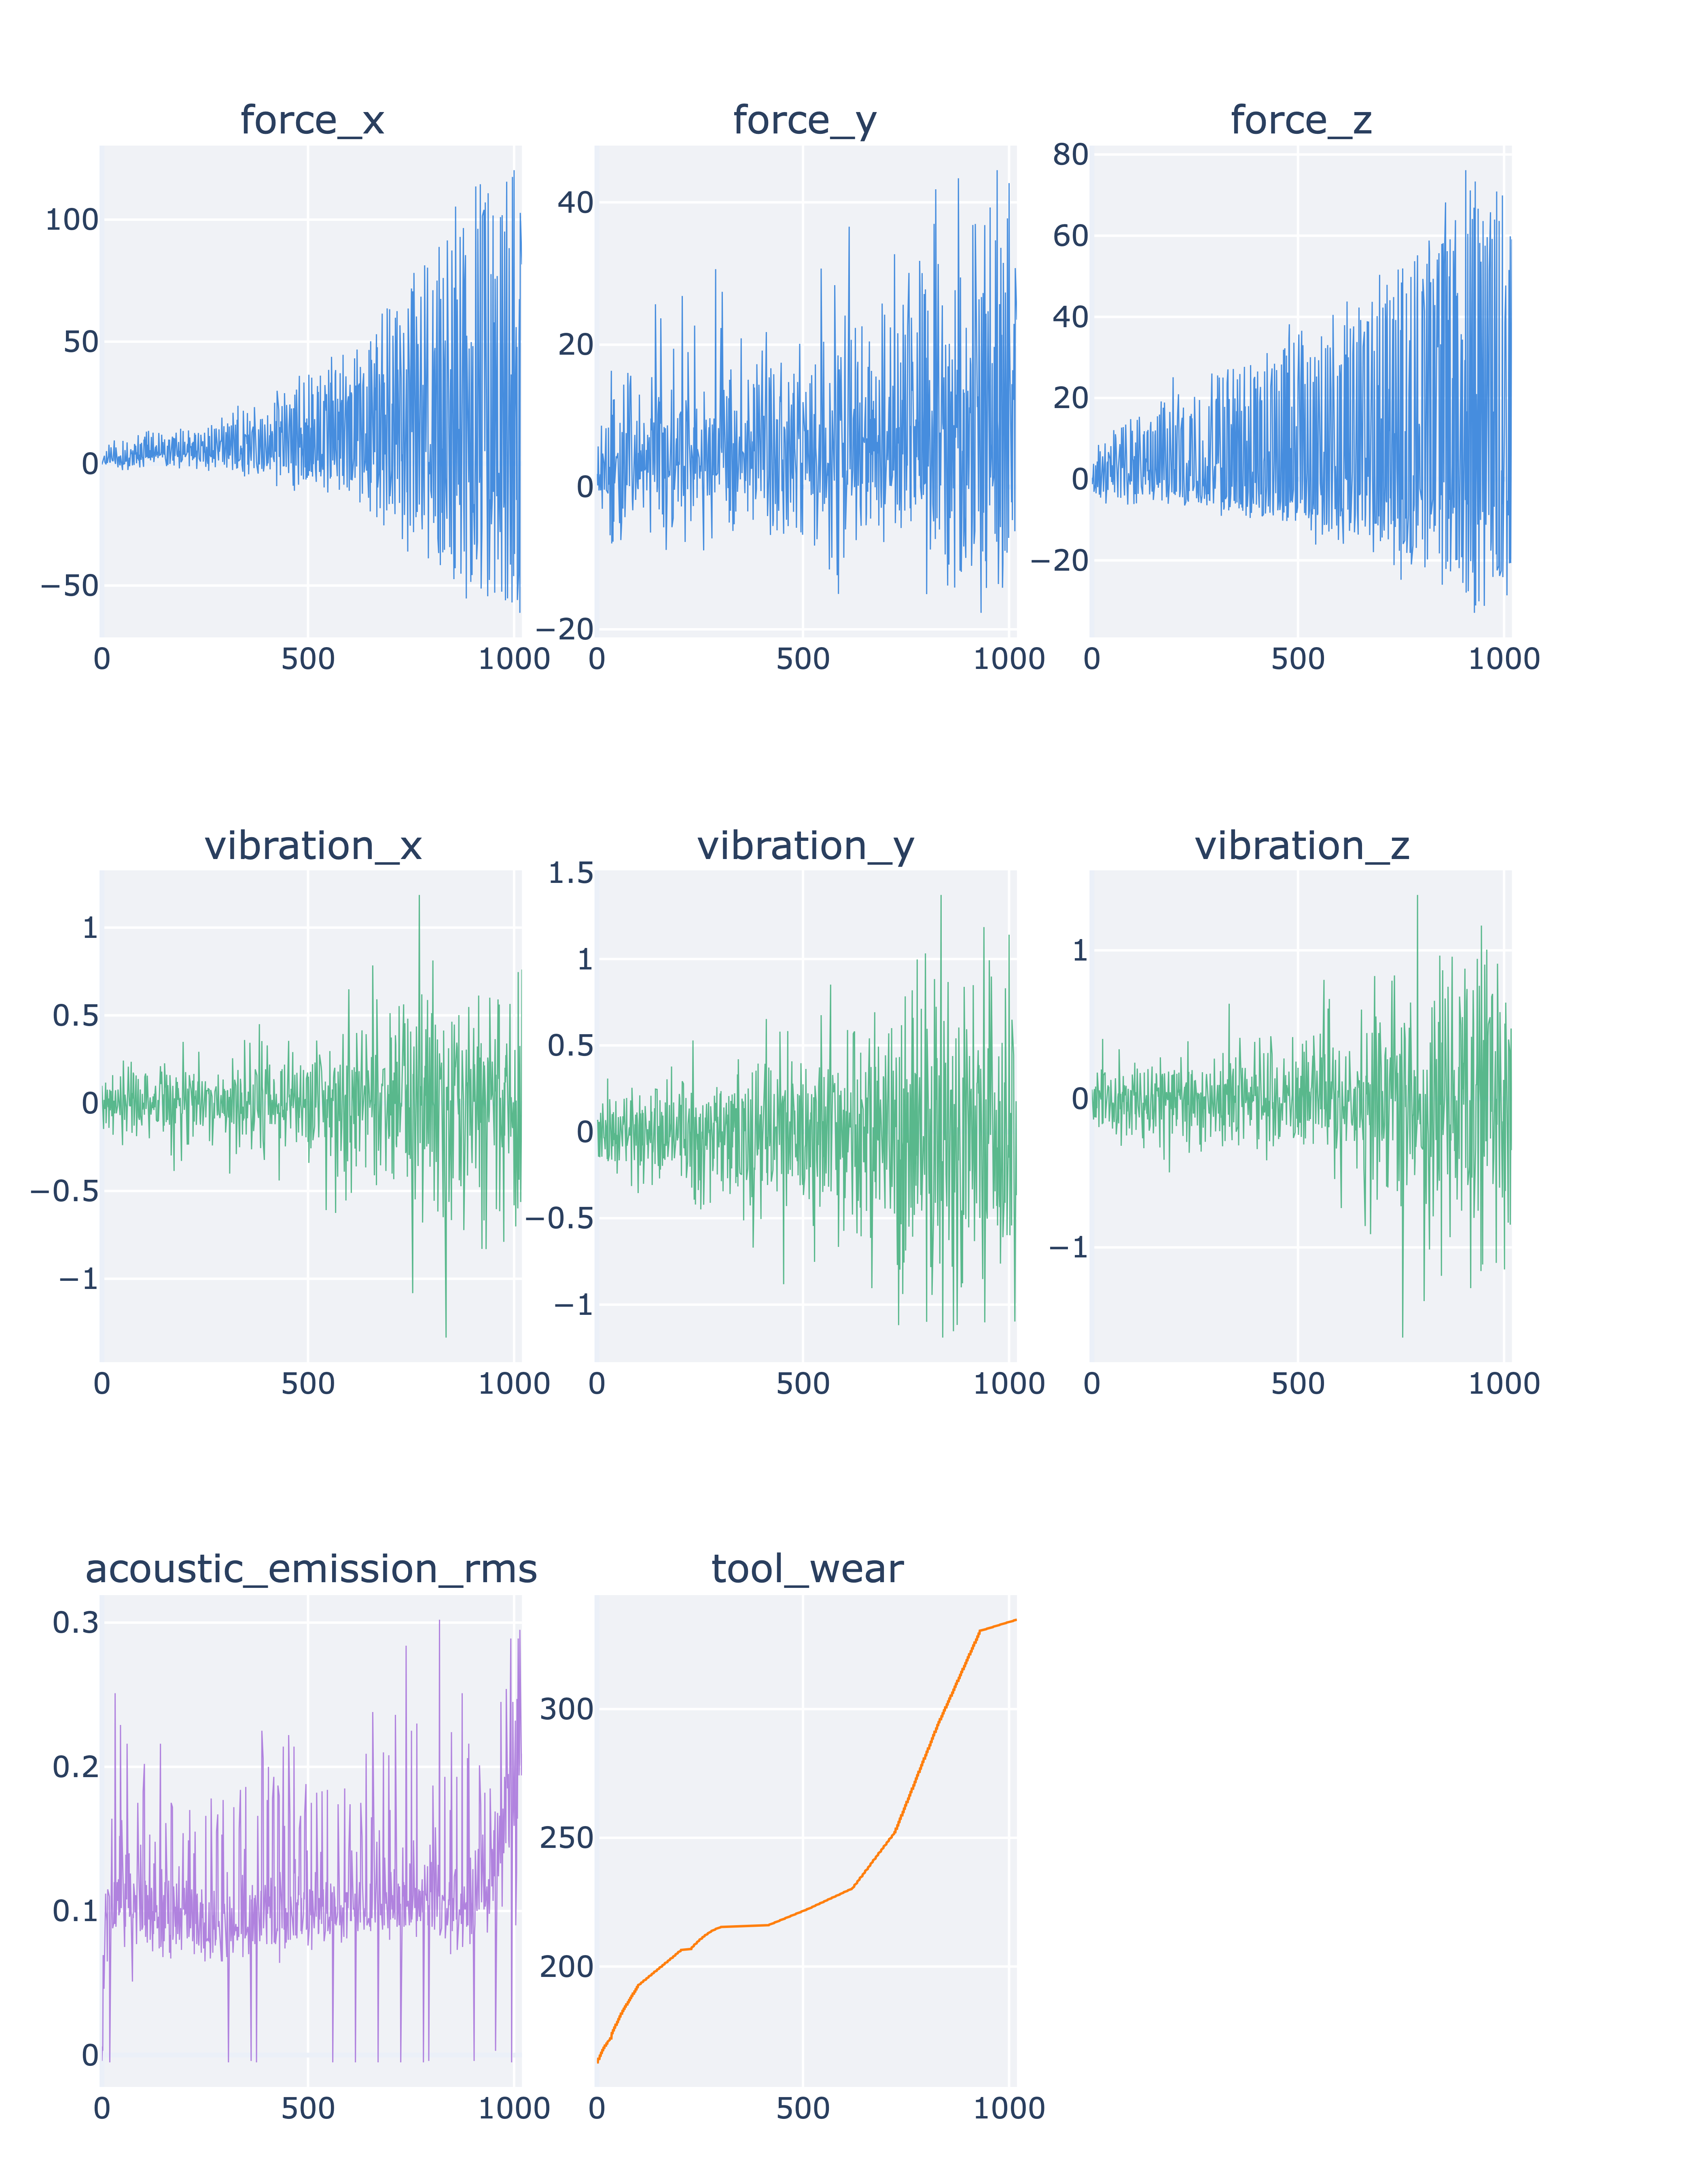
\includegraphics[width=\linewidth]{IEEE_06_SensorPlot.png}
		\caption{IEEE schema features.}
		\label{fig:schema_ieee}
	\end{subfigure}\hfill
	\begin{subfigure}[t]{0.48\textwidth}
		\centering
		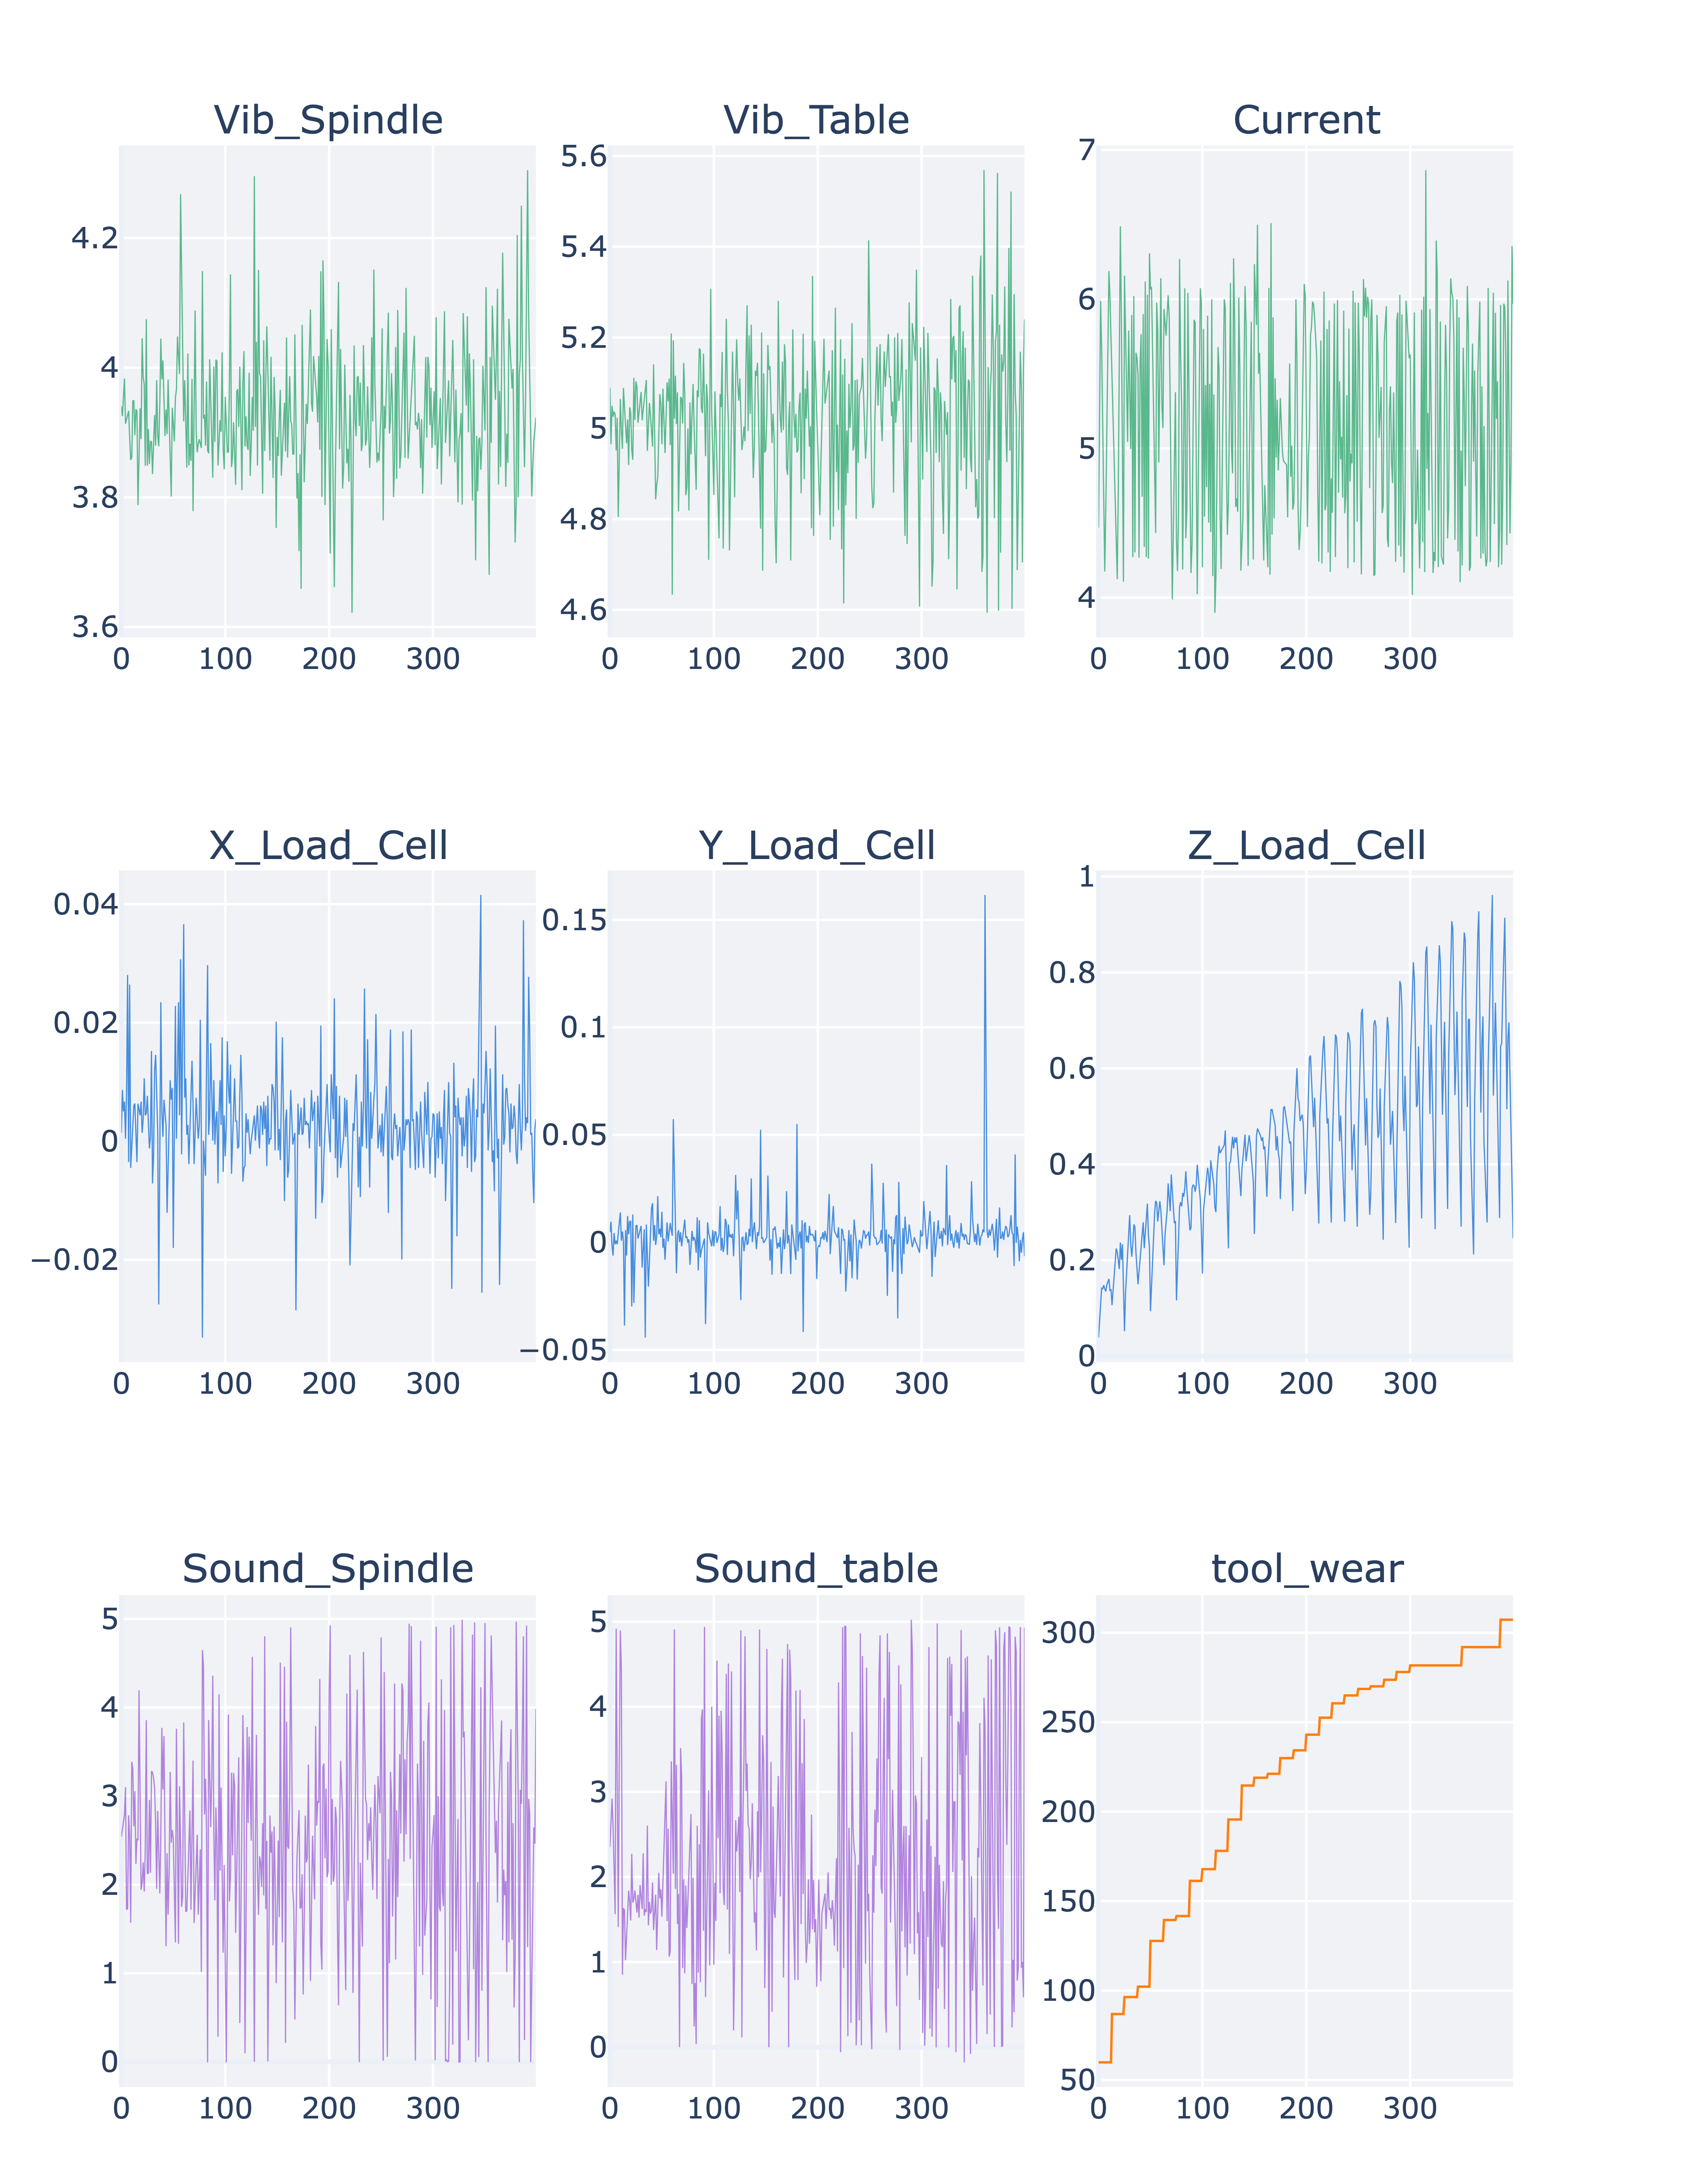
\includegraphics[width=\linewidth]{SIT_20_SensorPlot.png}
		\caption{SIT schema features.}
		\label{fig:schema_sit}
	\end{subfigure}
	\caption{Representative IEEE and SIT sensor traces showing schema differences.}
	\label{fig:schema_feature_plots_ieee_sit}
\end{figure}

\begin{figure}[htbp!]
	\centering
	\begin{subfigure}[t]{0.7\textwidth}
		\centering
		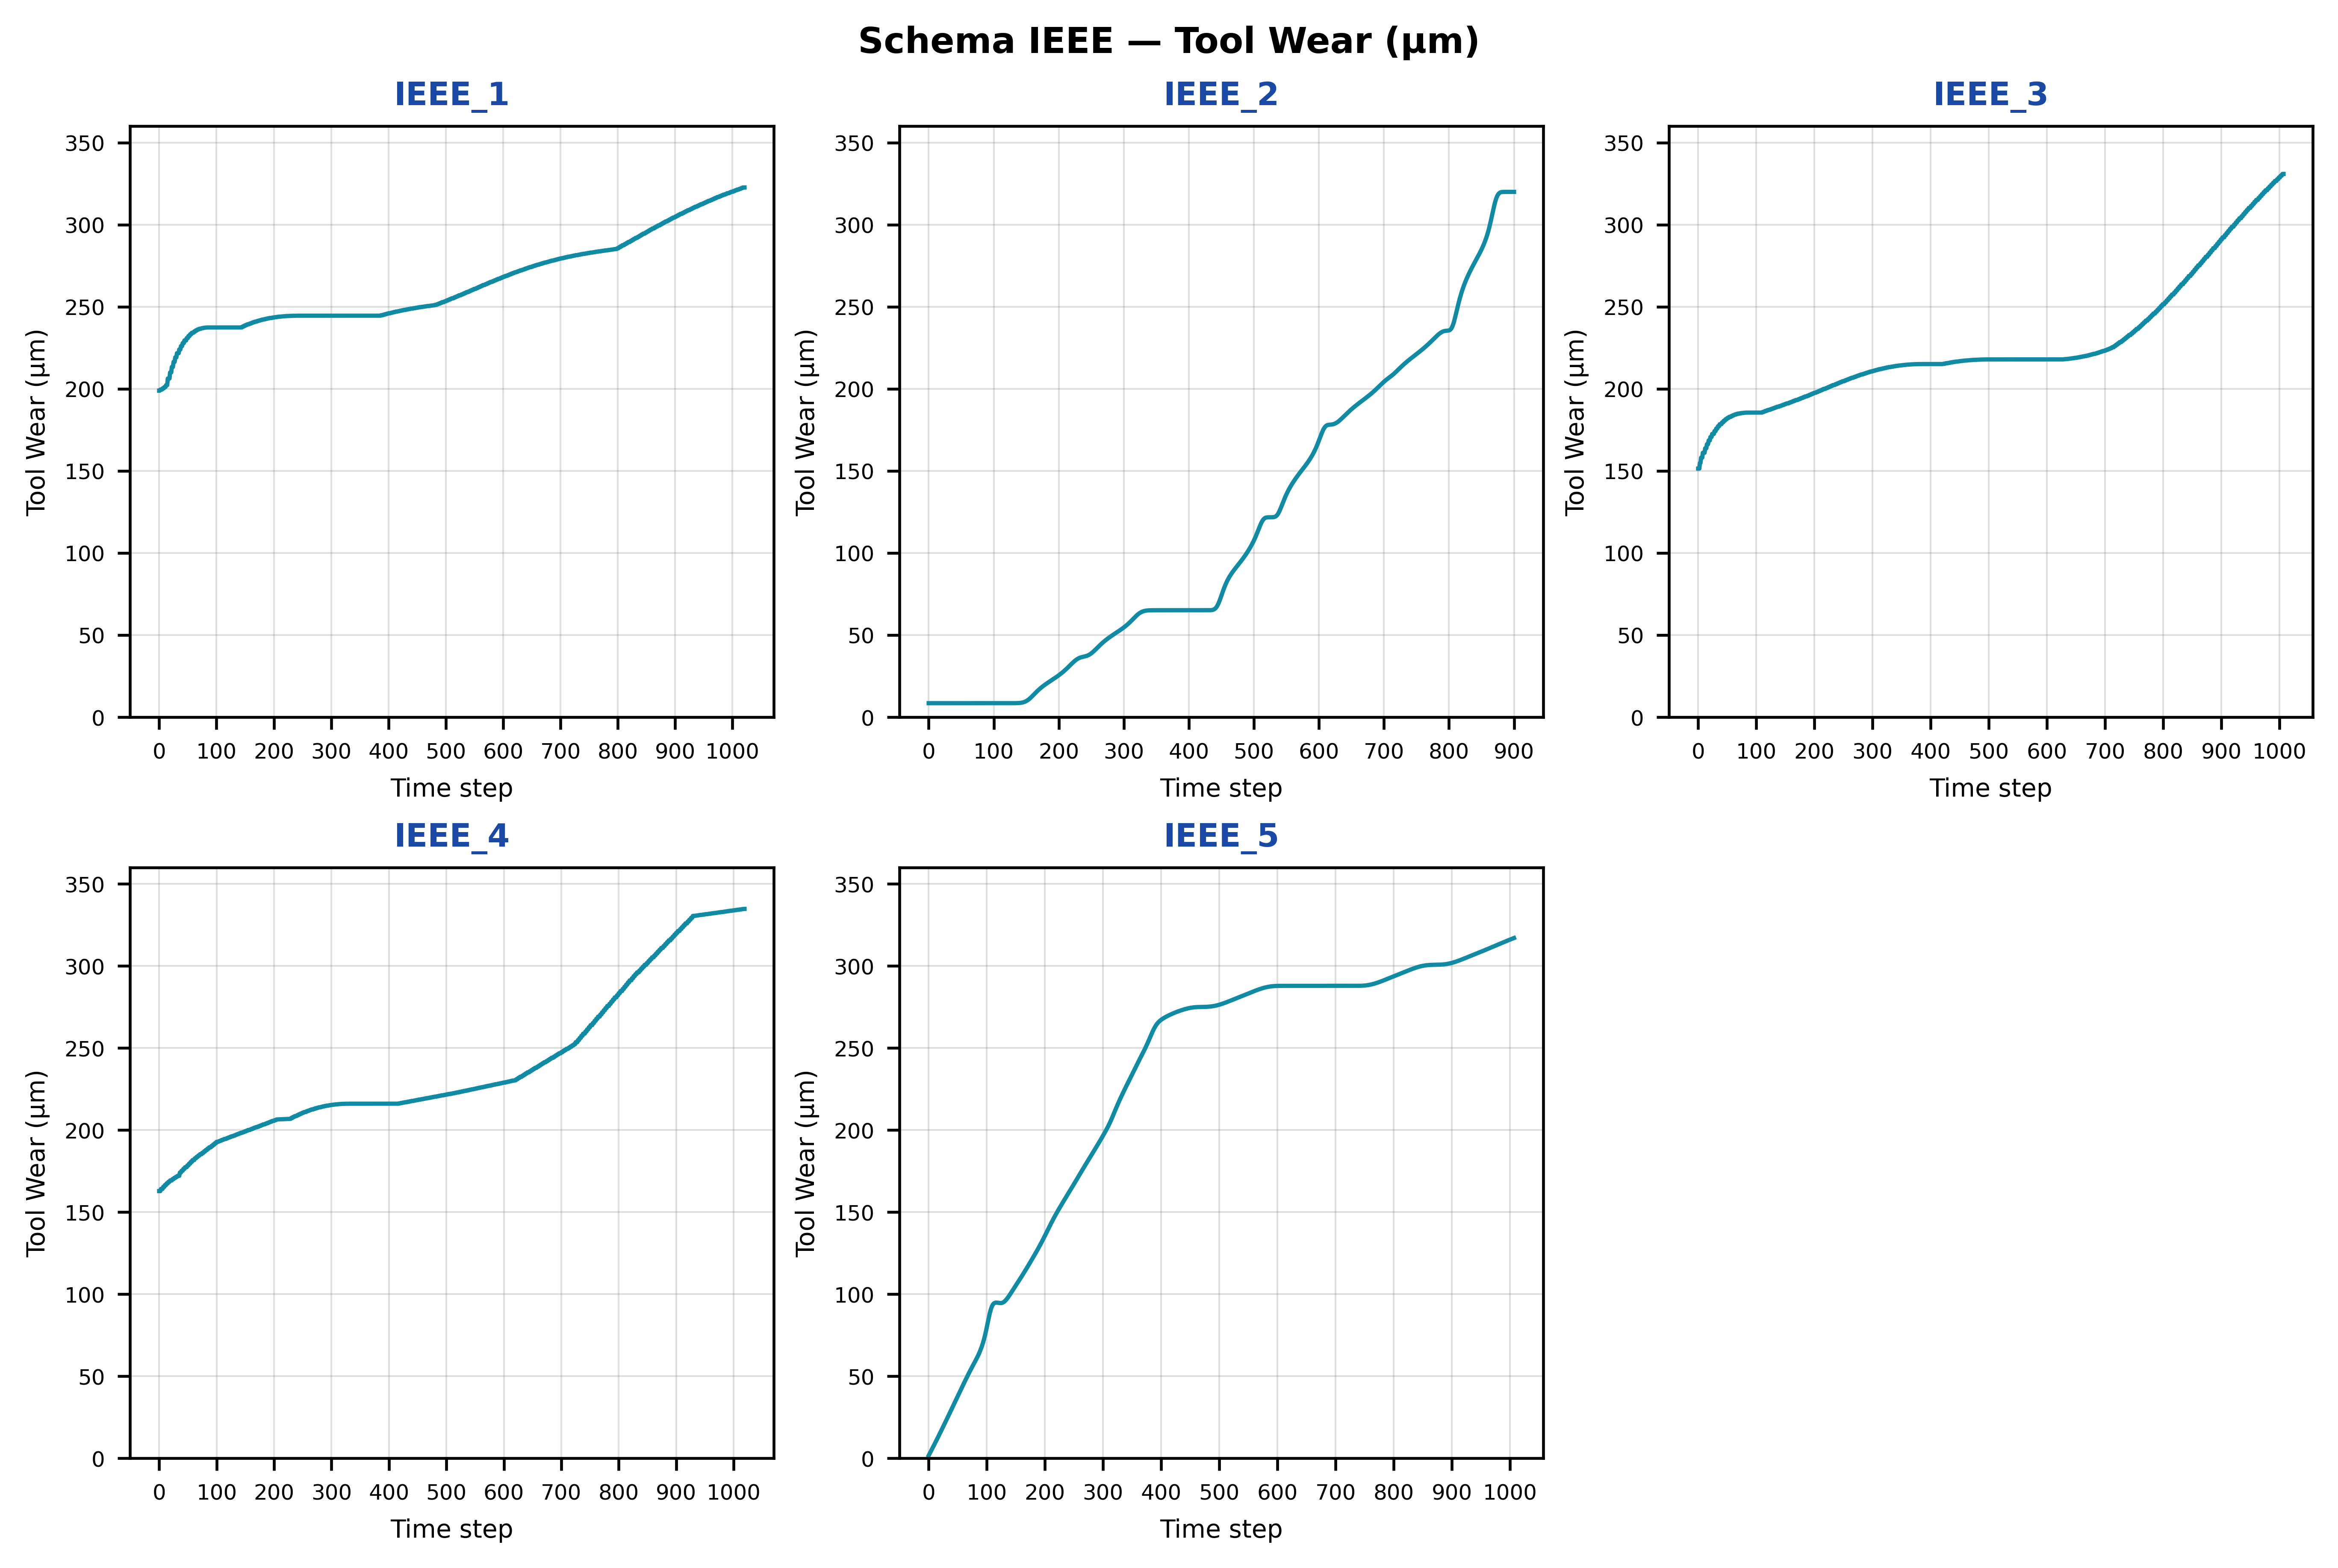
\includegraphics[width=\linewidth]{Tool_wear_IEEE.png}
		\caption{IEEE dataset tool wear plots.}
		\label{fig:schema_tw_ieee}
	\end{subfigure}
	\begin{subfigure}[t]{0.7\textwidth}
		\centering
		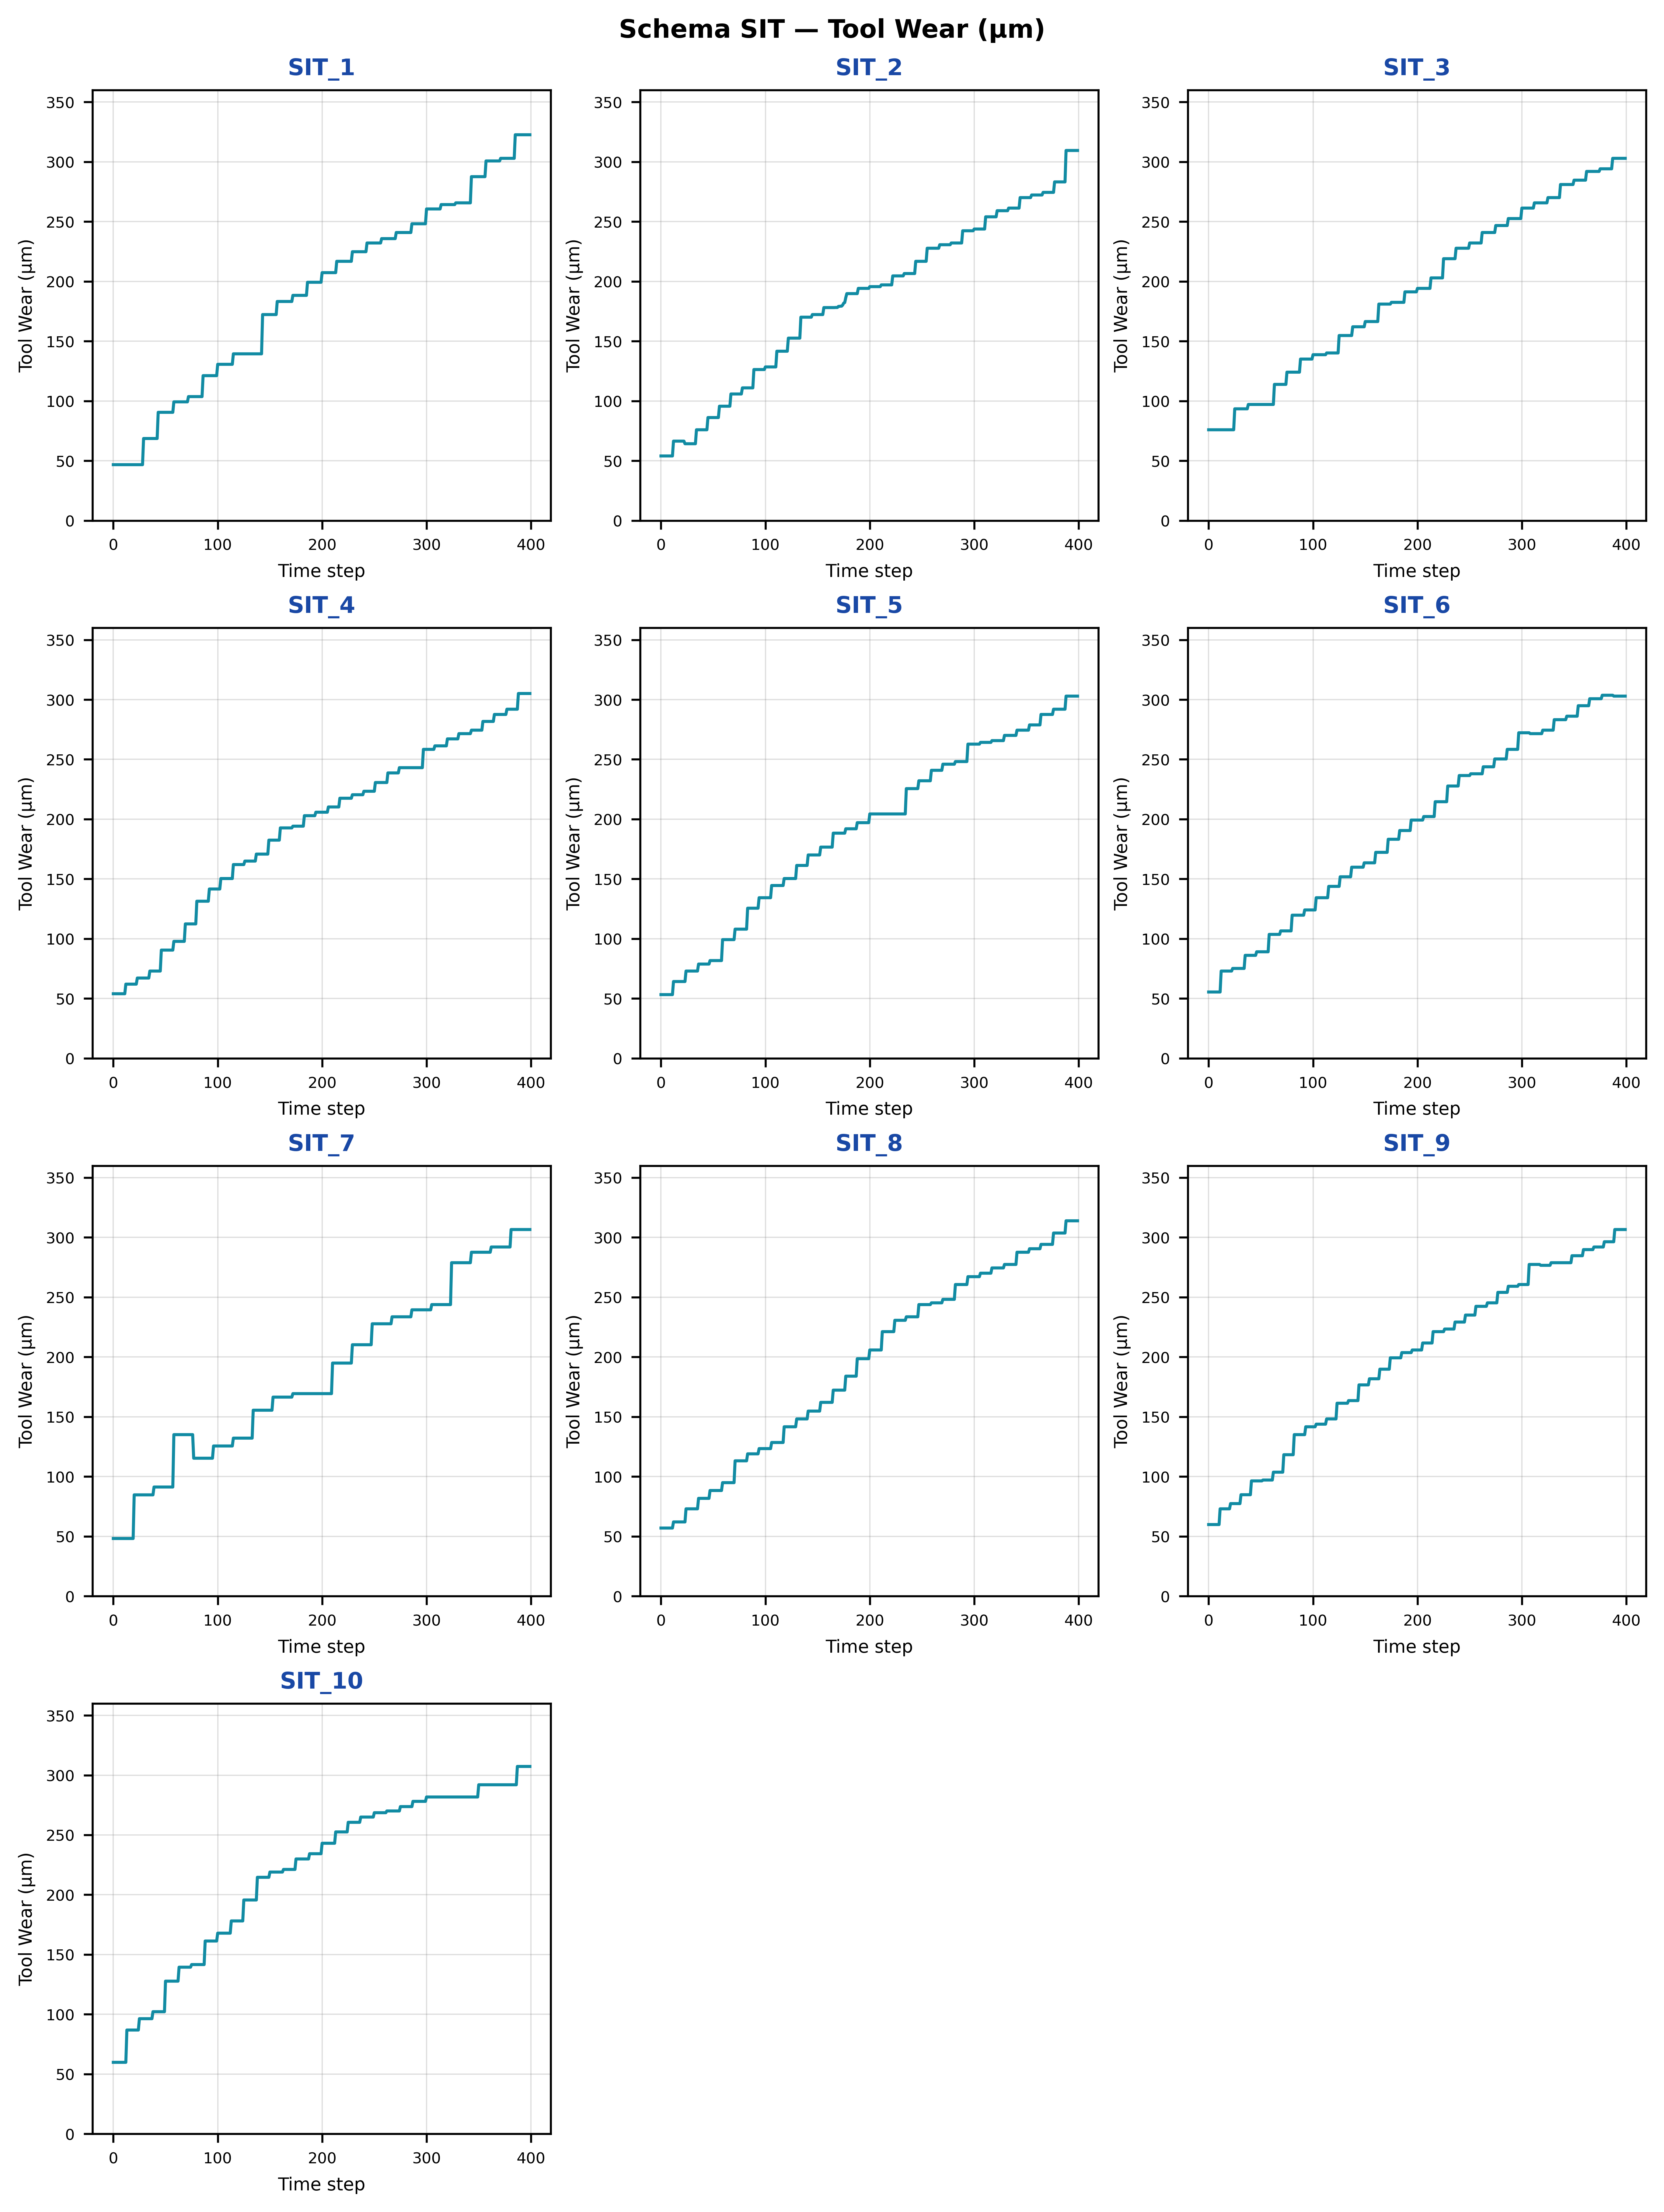
\includegraphics[width=\linewidth]{Tool_wear_SIT.png}
		\caption{SIT dataset tool wear plots.}
		\label{fig:schema_tw_sit}
	\end{subfigure}
	\caption{IEEE and SIT tool wear plots - showing schema differences.}
	\label{fig:schema_tool_wear_ieee_sit}
\end{figure}

\paragraph{IEEE benchmark dataset:}
The IEEE dataset \cite{PHMdata2010} comes from the PHM Society 2010 Data Challenge for high-speed CNC milling. We use seven channels from the release format: three-axis cutting force, three-axis vibration, and acoustic-emission RMS. Five files are used in the experiments.

\paragraph{SIT in-house dataset (university milling testbed):}
The SIT dataset is collected on a Vertical Milling Centre (Jyoti NVU PX10) using an NI data acquisition system. Tool wear is measured with a tool-makers microscope. The experiments span spindle speeds of 800--1{,}200~rpm and feed rates of 20--40~mm/min, with measured flank wear, denoted by \textsc{VB}, up to 0.32~mm. The eight-channel SIT schema contains spindle/table vibration, spindle/table sound, three-axis load-cell signals, and spindle current. Figure~\ref{fig:schema_feature_plots_ieee_sit} shows representative IEEE and SIT sensor traces. Figure~\ref{fig:schema_tool_wear_ieee_sit} shows the variation in tool wear for all IEEE and SIT datasets used.

\textbf{Differences between schemas:}
The schemas differ in channel count and sensor type. IEEE uses force, vibration, and acoustic emission; SIT uses vibration, sound, load, and current. The environment changes only the sensor set.

\paragraph{Datasets and train/test protocol:}
Each model is trained on one wear-cycle file and evaluated on the remaining unseen files from the same schema. 

\paragraph{Baselines and metrics:}
\label{sec:metrics}
The main comparison is among RL agents using raw sensor observations. Conventional supervised-ML baselines are not included because they require task-specific feature engineering and were not considered suitable for an AutoRL workflow. Therefore our scope of study covers only RL baselines.

\paragraph{Evaluation metrics:}
To compare the models, we developed simple metrics focused on practitioner requirements. We compute a model comparison score $\mathrm{S}$ and a replacement timing metric $\lambda$.

\paragraph{The Lambda metric for prognostic evaluation, $\lambda$:}

\begin{figure}[htbp!]
	\centering
	\includegraphics[width=\linewidth]{LambdaPlot.png}
	\caption{The Lambda metric for prognostic evaluation.}
	\label{fig:Lambda}
\end{figure}

Inspired by prognostic-specific metrics \cite{Saxena2010Metrics}, we define a timing metric $t_{\lambda}$ displayed in Figure \ref{fig:Lambda}:
\begin{equation}
		\lambda = t_{\mathrm{WT}} - t_{\mathrm{FR}},
\end{equation}
where $t_{\mathrm{FR}}$ is the timestep where the agent suggested the \emph{first} tool maintenance action, and $t_{\mathrm{WT}}$ is the threshold timestep.
An ideal value for $\lambda$ is zero; a small positive value indicates replacement before hitting the threshold, while a small negative value indicates replacement after the threshold.

\paragraph{The model evaluation score, $\mathrm{S}$:}
$\tau$ is the configured wear threshold and $t_{\mathrm{WT}}$ the timestep at which this threshold is crossed. $T_\mathrm{RM}$ is the allowable replacement margin. Let $W_1, W_2, W_3$ be the weightages assigned to tool life usage $u$, timing of replacement $\lambda$, and threshold violations $v$, respectively.

The fraction of tool usage, $u\in(0,1]$, is computed as per equation (\ref{eq:u}). Let $v\in\mathbb{N}_0$ be the number of threshold violations, computed when the model suggests continuation beyond the threshold timesteps without having made a replacement suggestion yet. Equation (\ref{eq:tim}) ensures that large $\lambda$ values are penalized and values clipped to ensure they remain within $[0,1]$.

The evaluation score $\mathrm{S}$ is computed as follows:

\begin{align}
	u &= \min\left(\frac{t_{\mathrm{FR}}}{t_{\mathrm{WT}}},\, 1.0\right) \label{eq:u}\\
	S_{\text{tool-life}} &= u,\\
	S_{\lambda} &= \max\left(0,\,1-\frac{|\lambda|}{T_{\mathrm{RM}}}\right), \label{eq:tim}\\
	S_{\text{violations}} &= \frac{1}{1+v},\\
	S &= W_1 \times S_{\text{tool-life}} + W_2 \times S_{\lambda} + W_3 \times S_{\text{violations}} \label{eq:S}.
\end{align}

$\tau$ is the configured wear threshold (default setting is $300\,\mu\mathrm{m}$) and $T_{\mathrm{RM}}$ is an allowable replacement margin (default setting is 5\% on either side of the wear threshold). We set the scoring component weightages as follows: $W_1 = 0.50$, $W_2 = 0.30$, and $W_3 = 0.20$. The AutoRL bench allows practitioners to override all defaults.

The score evaluates models based on operational parameters rather than RL-specific metrics such as average episode rewards, providing an explainable model selection metric.

\paragraph{Multi-round evaluation, confidence intervals, and exploratory hypothesis tests:}
SIT uses 20 evaluation rounds per held-out file to capture stochastic action variation. Welch tests are treated as exploratory because observations are nested within trained-model/held-out-file pairs. We report sample means and 95\% confidence intervals over held-out evaluations.

\section{Results} \label{sec:results}
For each schema, four RL algorithms are evaluated under a no-attention baseline alongside four distinct attention mechanisms: Nadaraya--Watson, temporal, self-attention, and multi-head.

\subsection{Main performance tables and focused statistical tests}
\label{sec:hypothesis_tests}

Tables~\ref{tab:sit_main_results} and \ref{tab:ieee_main_results} report the mean $\pm$ standard deviation of evaluation scores across the SIT and IEEE schemas. Table~\ref{tab:rf_vs_ppo_tests} summarizes the focused one-tailed Welch $t$-tests evaluating the hypothesis \textsc{REINFORCE} $>$ \textsc{PPO}. 

\begin{table}[htbp]
	\centering
	\caption{SIT schema: mean $\pm$ std. dev. evaluation score.}
	\label{tab:sit_main_results}
	\begin{tabular}{l l l l l l}
	\toprule
	\textbf{RL Algo} & \textbf{Baseline} & \textbf{Nadaraya--Watson} & \textbf{Temporal} & \textbf{Self-attention} & \textbf{Multi-head}\\
	\midrule
	A2C & 0.2456 $\pm$ 0.0043 & 0.2456 $\pm$ 0.0043 & 0.2456 $\pm$ 0.0043 & \textbf{0.3130 $\pm$ 0.2040} & 0.2456 $\pm$ 0.0043\\
	DQN & 0.2456 $\pm$ 0.0043 & 0.2456 $\pm$ 0.0043 & 0.2456 $\pm$ 0.0043 & 0.2456 $\pm$ 0.0043 & 0.2456 $\pm$ 0.0043\\
	PPO & 0.6313 $\pm$ 0.3347 & 0.7132 $\pm$ 0.3172 & 0.5771 $\pm$ 0.3337 & 0.6089 $\pm$ 0.3305 & \textbf{0.8004 $\pm$ 0.2694}\\
	REINFORCE & 0.4907 $\pm$ 0.3108 & \textbf{0.8646 $\pm$ 0.2032} & 0.6406 $\pm$ 0.3355 & 0.6997 $\pm$ 0.3171 & 0.7917 $\pm$ 0.2738\\
	\bottomrule
	\end{tabular}
\end{table}

\begin{table}[htbp]
	\centering
	\caption{IEEE schema: mean $\pm$ std. dev. evaluation score.}
	\label{tab:ieee_main_results}
	\begin{tabular}{l l l l l l}
	\toprule
	\textbf{RL Algo} & \textbf{Baseline} & \textbf{Nadaraya--Watson} & \textbf{Temporal} & \textbf{Self-attention} & \textbf{Multi-head}\\
	\midrule
	A2C & 0.6180 $\pm$ 0.2640 & 0.4322 $\pm$ 0.2753 & 0.3565 $\pm$ 0.2496 & 0.2729 $\pm$ 0.1281 & \textbf{0.7424 $\pm$ 0.2695}\\
	DQN & \textbf{0.5996 $\pm$ 0.2550} & 0.2360 $\pm$ 0.0016 & 0.2360 $\pm$ 0.0016 & 0.2360 $\pm$ 0.0016 & 0.2878 $\pm$ 0.1811\\
	PPO & 0.7484 $\pm$ 0.1418 & \textbf{0.8343 $\pm$ 0.1867} & 0.7608 $\pm$ 0.2641 & 0.8044 $\pm$ 0.2174 & 0.8232 $\pm$ 0.1870\\
	REINFORCE & 0.6696 $\pm$ 0.2214 & 0.8008 $\pm$ 0.2186 & 0.8848 $\pm$ 0.0737 & \textbf{0.8860 $\pm$ 0.0708} & 0.8559 $\pm$ 0.1443\\
	\bottomrule
	\end{tabular}
\end{table}

\begin{table}[htbp]
	\centering
	\caption{Focused one-tailed Welch tests for \textsc{REINFORCE} $>$ \textsc{PPO} at $\alpha=0.05$.}
	\label{tab:rf_vs_ppo_tests}
	\begin{tabular}{l l r r l}
	\toprule
	\textbf{Schema} & \textbf{Setting} & \textbf{t-stat} & \textbf{p-value} & \textbf{Supported?}\\
	\midrule
	SIT & Baseline (no attention) & -2.9224 & 0.9980 & No\\
	SIT & With attention (pooled) & \textbf{3.1941} & \textbf{0.0007} & \textbf{Yes}\\
	IEEE & Baseline (no attention) & -1.3409 & 0.9053 & No\\
	IEEE & With attention (pooled) & \textbf{1.9865} & \textbf{0.0243} & \textbf{Yes}\\
	\bottomrule
	\end{tabular}
\end{table}

\paragraph{Algorithm hierarchy reversal:}
Without attention, \textsc{PPO} achieves the highest mean evaluation score in both schemas (SIT: $0.6313$; IEEE: $0.7484$). However, when integrated with optimal attention features, \textsc{REINFORCE} leapfrogs \textsc{PPO} to achieve the highest overall mean scores (SIT: $0.7492$ pooled, peaking at \textbf{0.8646} with Nadaraya--Watson; IEEE: $0.8569$ pooled, peaking at \textbf{0.8860} with self-attention). As shown in Table~\ref{tab:rf_vs_ppo_tests}, the hypothesis that \textsc{REINFORCE} outperforms \textsc{PPO} is unsupported at baseline ($p > 0.90$ across schemas) but becomes strongly supported under attention augmentation (SIT: $t = 3.1941, p = 0.0007$; IEEE: $t = 1.9865, p = 0.0243$).

\paragraph{Mechanism-level synthesis for \textsc{REINFORCE} and \textsc{PPO}:}
Table~\ref{tab:best_mech_ppo_rf} highlights the optimal attention mechanism for policy gradient architectures. In SIT, \textsc{REINFORCE} performs best with Nadaraya--Watson (\textbf{0.8646 $\pm$ 0.2032}), while \textsc{PPO} reaches its peak under multi-head attention (\textbf{0.8004 $\pm$ 0.2694}). In IEEE, \textsc{REINFORCE} achieves optimal performance with self-attention (\textbf{0.8860 $\pm$ 0.0708}), whereas \textsc{PPO} peaks under Nadaraya--Watson (\textbf{0.8343 $\pm$ 0.1867}).

\begin{table}[htbp]
\centering
	\caption{Best attention mechanism by schema for \textsc{REINFORCE} and \textsc{PPO} (mean $\pm$ std. dev. evaluation score).}
	\label{tab:best_mech_ppo_rf}
	\begin{tabular}{l l l l}
	\toprule
	\textbf{Schema} & \textbf{Algorithm} & \textbf{Best attention mechanism} & \textbf{Eval. score (mean $\pm$ std. dev.)}\\
	\midrule
	SIT & \textsc{REINFORCE} & Nadaraya--Watson & \textbf{0.8646 $\pm$ 0.2032}\\
	SIT & \textsc{PPO} & Multi-head & \textbf{0.8004 $\pm$ 0.2694}\\
	IEEE & \textsc{REINFORCE} & Self-attention & \textbf{0.8860 $\pm$ 0.0708}\\
	IEEE & \textsc{PPO} & Nadaraya--Watson & \textbf{0.8343 $\pm$ 0.1867}\\
	\bottomrule
	\end{tabular}
\end{table}

\subsection{Ablation study and the "Algorithm Masking" effect} \label{sec:ablation_results}

Table~\ref{tab:ablation_condensed} provides a condensed ablation analysis across algorithmic groupings and individual setups.

\begin{table}[htbp]
	\centering
	\caption{Condensed ablation study analysis (one-tailed Welch t-tests vs. baseline).}
	\label{tab:ablation_condensed}
	\begin{tabular}{l l r r r r}
		\toprule
		\textbf{Schema} & \textbf{Comparison} & \textbf{No attn.} & \textbf{Attention} & \textbf{t-stat} & \textbf{$p$ (1-tail)}\\
		\midrule
		SIT & \textsc{REINFORCE} only & 0.4907 & \textbf{0.7492} & \textbf{7.1139} & \textbf{0.0000}\\
		IEEE & \textsc{REINFORCE} only & 0.6696 & \textbf{0.8569} & \textbf{3.6351} & \textbf{0.0007}\\
		SIT & PPO + \textsc{REINFORCE}, pooled & 0.5610 & \textbf{0.7120} & \textbf{5.5498} & \textbf{0.0000}\\
		IEEE & PPO + \textsc{REINFORCE}, pooled & 0.7090 & \textbf{0.8313} & \textbf{3.7724} & \textbf{0.0002}\\
		SIT & All algorithms, pooled & 0.4033 & \textbf{0.4830} & \textbf{4.6626} & \textbf{0.0000}\\
		IEEE & All algorithms, pooled & \textbf{0.6589} & 0.5906 & -2.2584 & 0.9873\\
		\bottomrule
	\end{tabular}
\end{table}

A critical empirical pattern is the \emph{Algorithm Masking Effect} observed in the IEEE schema. When evaluating all four algorithms in aggregate on IEEE, attention appears to reduce overall performance ($0.6589 \rightarrow 0.5906, t = -2.2584, p = 0.9873$). However, this aggregate signal is driven by the poor performance of value-based methods (\textsc{DQN} drops from $0.5996$ to $0.2360$) and actor-critic instability in \textsc{A2C} ($0.6180 \rightarrow 0.4510$). 

Once policy gradient architectures (\textsc{PPO} + \textsc{REINFORCE}) are isolated, attention mechanisms demonstrate robust, statistically significant performance enhancements across both schemas:
\begin{itemize}
    \item \textbf{SIT Schema:} Pooled policy gradient performance increases from $0.5610$ to \textbf{0.7120} ($t = 5.5498, p = 0.0000$).
    \item \textbf{IEEE Schema:} Pooled policy gradient performance increases from $0.7090$ to \textbf{0.8313} ($t = 3.7724, p = 0.0002$).
\end{itemize}

At the mechanism level, \textbf{Multi-Head Attention} emerges as the most universally robust feature extractor. It achieves the highest pooled score for policy-gradient algorithms in SIT (\textbf{0.7961}, $t = 7.3911, p = 0.0000$) and the second highest in IEEE (\textbf{0.8395}, $t = 3.4472, p = 0.0005$). Crucially, multi-head attention is the \emph{only} mechanism capable of stabilizing \textsc{A2C} in IEEE, elevating its score above baseline (\textbf{0.7424} vs. $0.6180, t = 1.5551$). Conversely, \textbf{Temporal Attention} yields the weakest gains, failing to achieve statistical significance for the pooled policy gradient group in SIT ($t = 1.3658, p = 0.0864$).

Figures~\ref{fig:analysis_reports}--\ref{fig:ablation_ppo_rf} illustrate the visual distributions corresponding to Tables~\ref{tab:sit_main_results}--\ref{tab:ablation_condensed}.

\begin{figure}[htbp!]
	\centering
	\begin{subfigure}{0.9\textwidth}
		\centering
		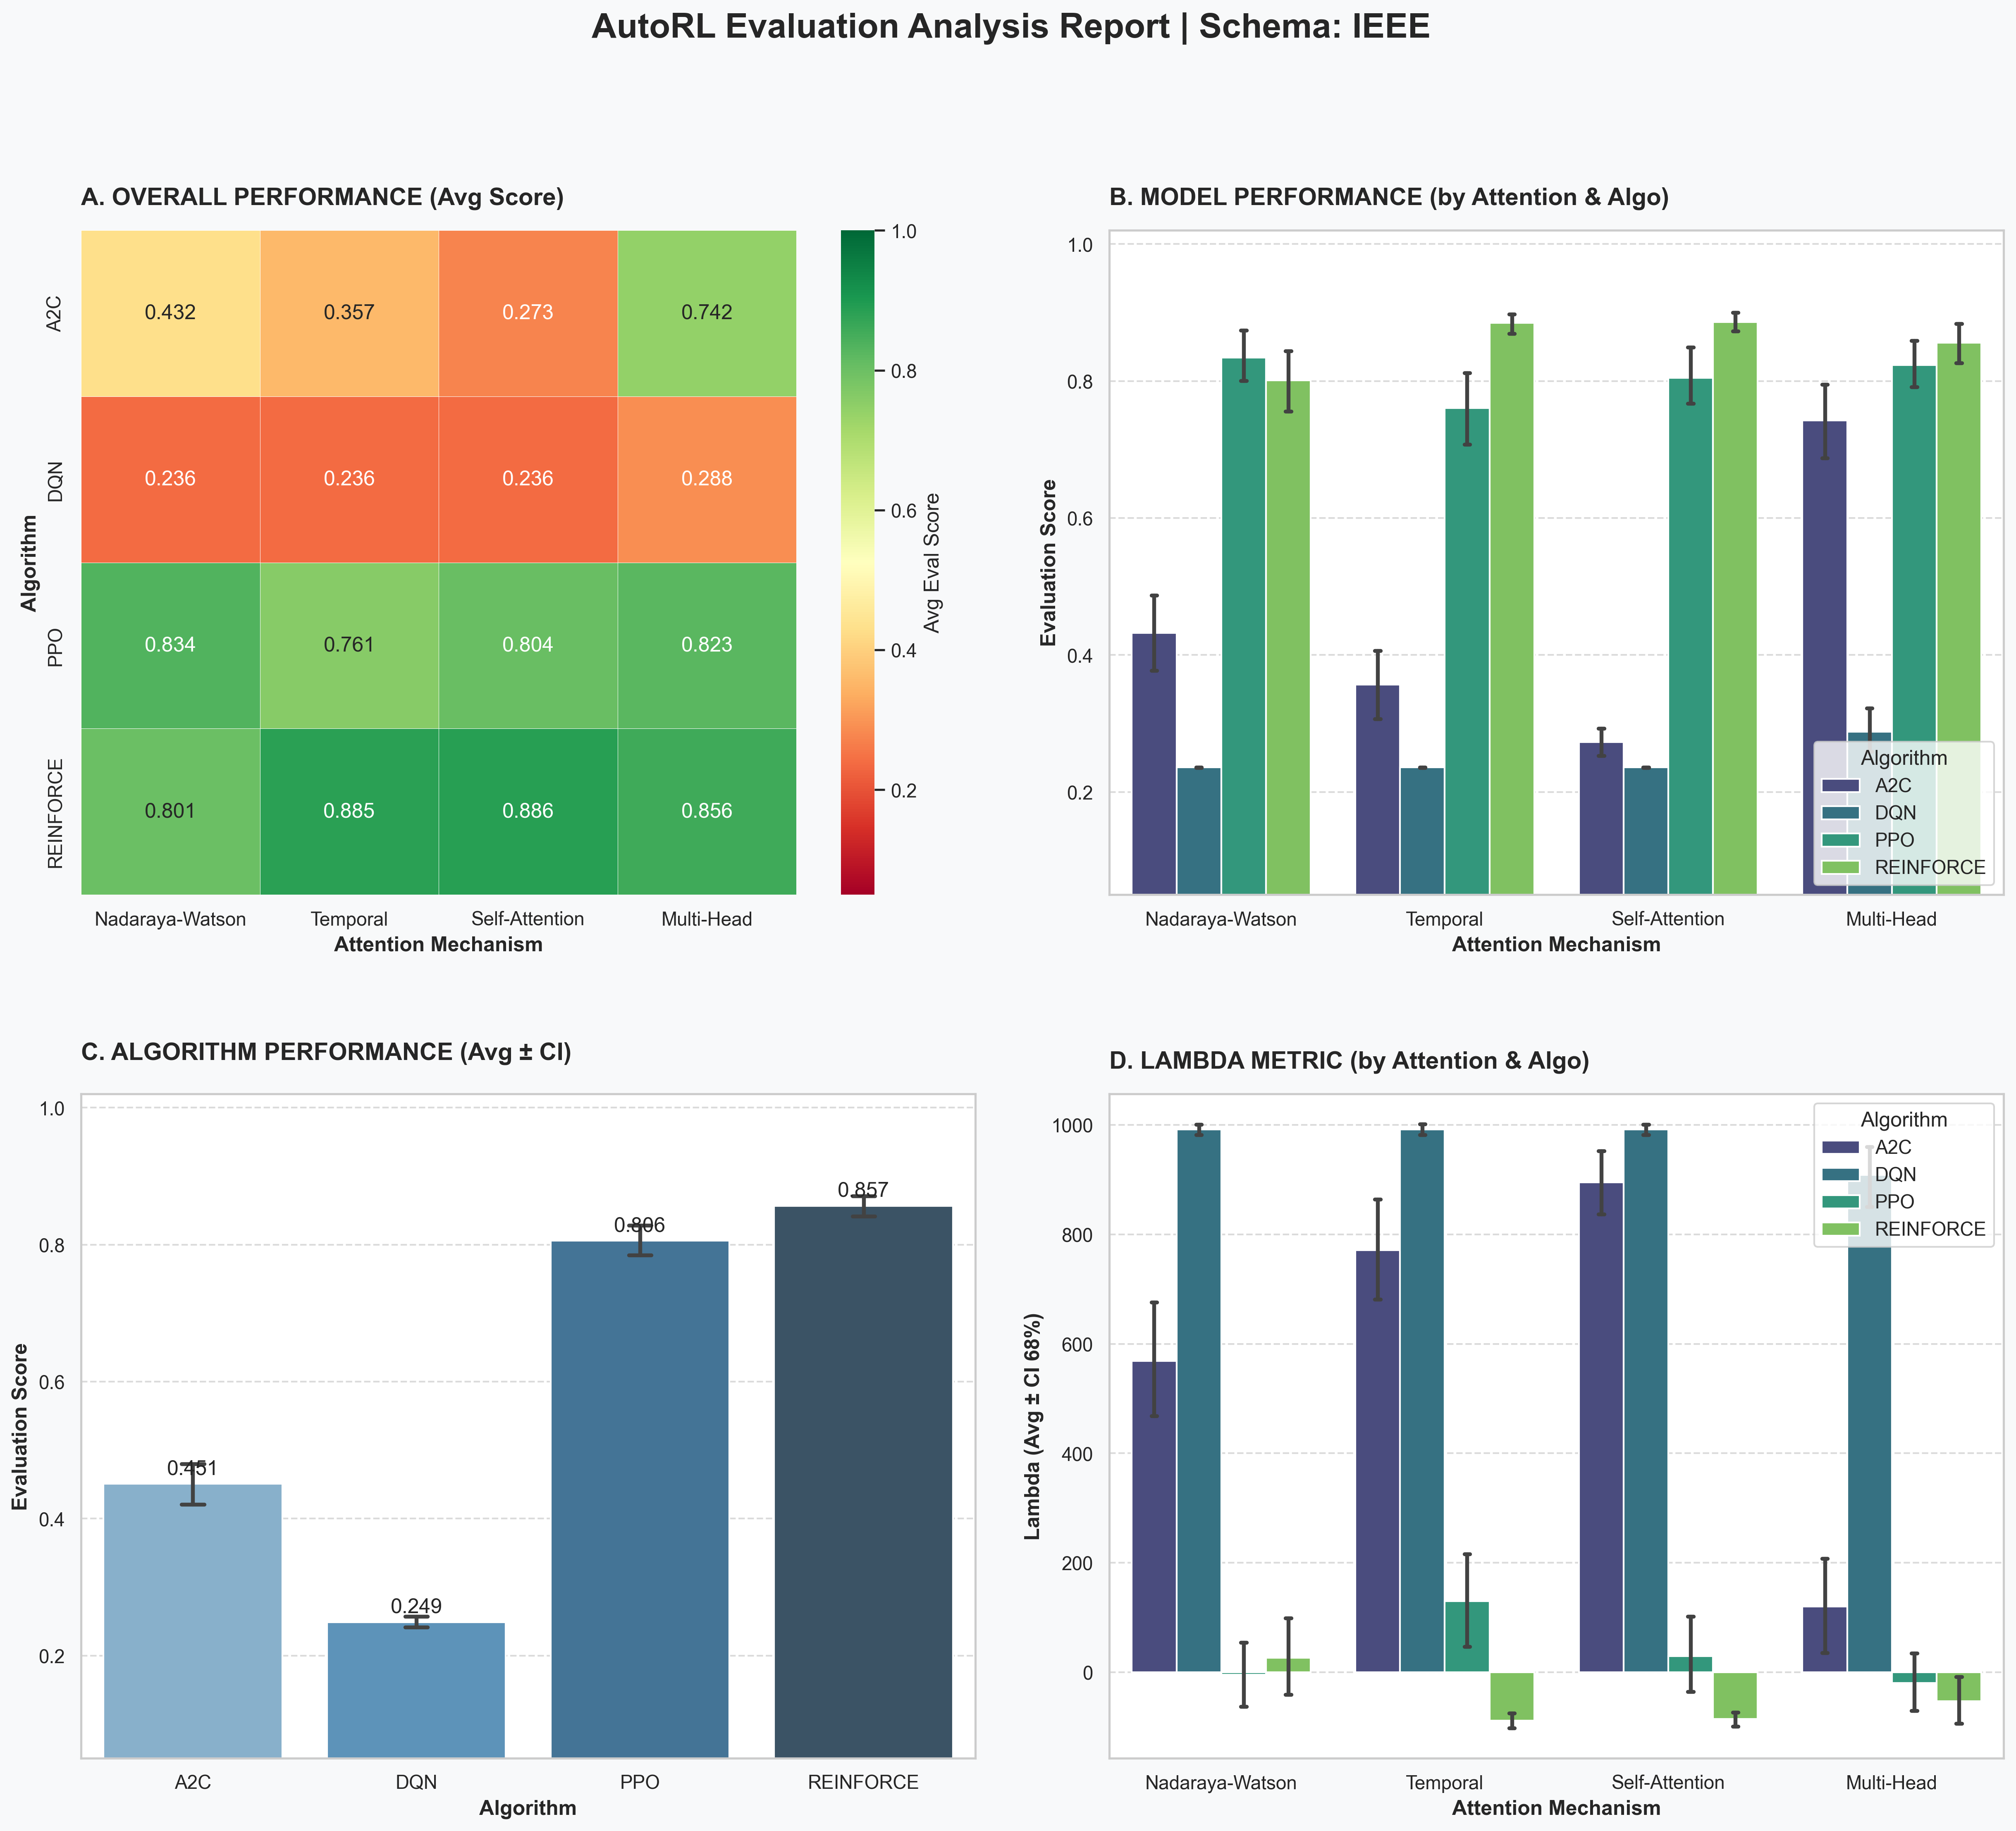
\includegraphics[width=\linewidth]{Analysis_Report_IEEE.png}
		\caption{IEEE analysis report.}
	\end{subfigure}
	
	\begin{subfigure}{0.9\textwidth}
		\centering
		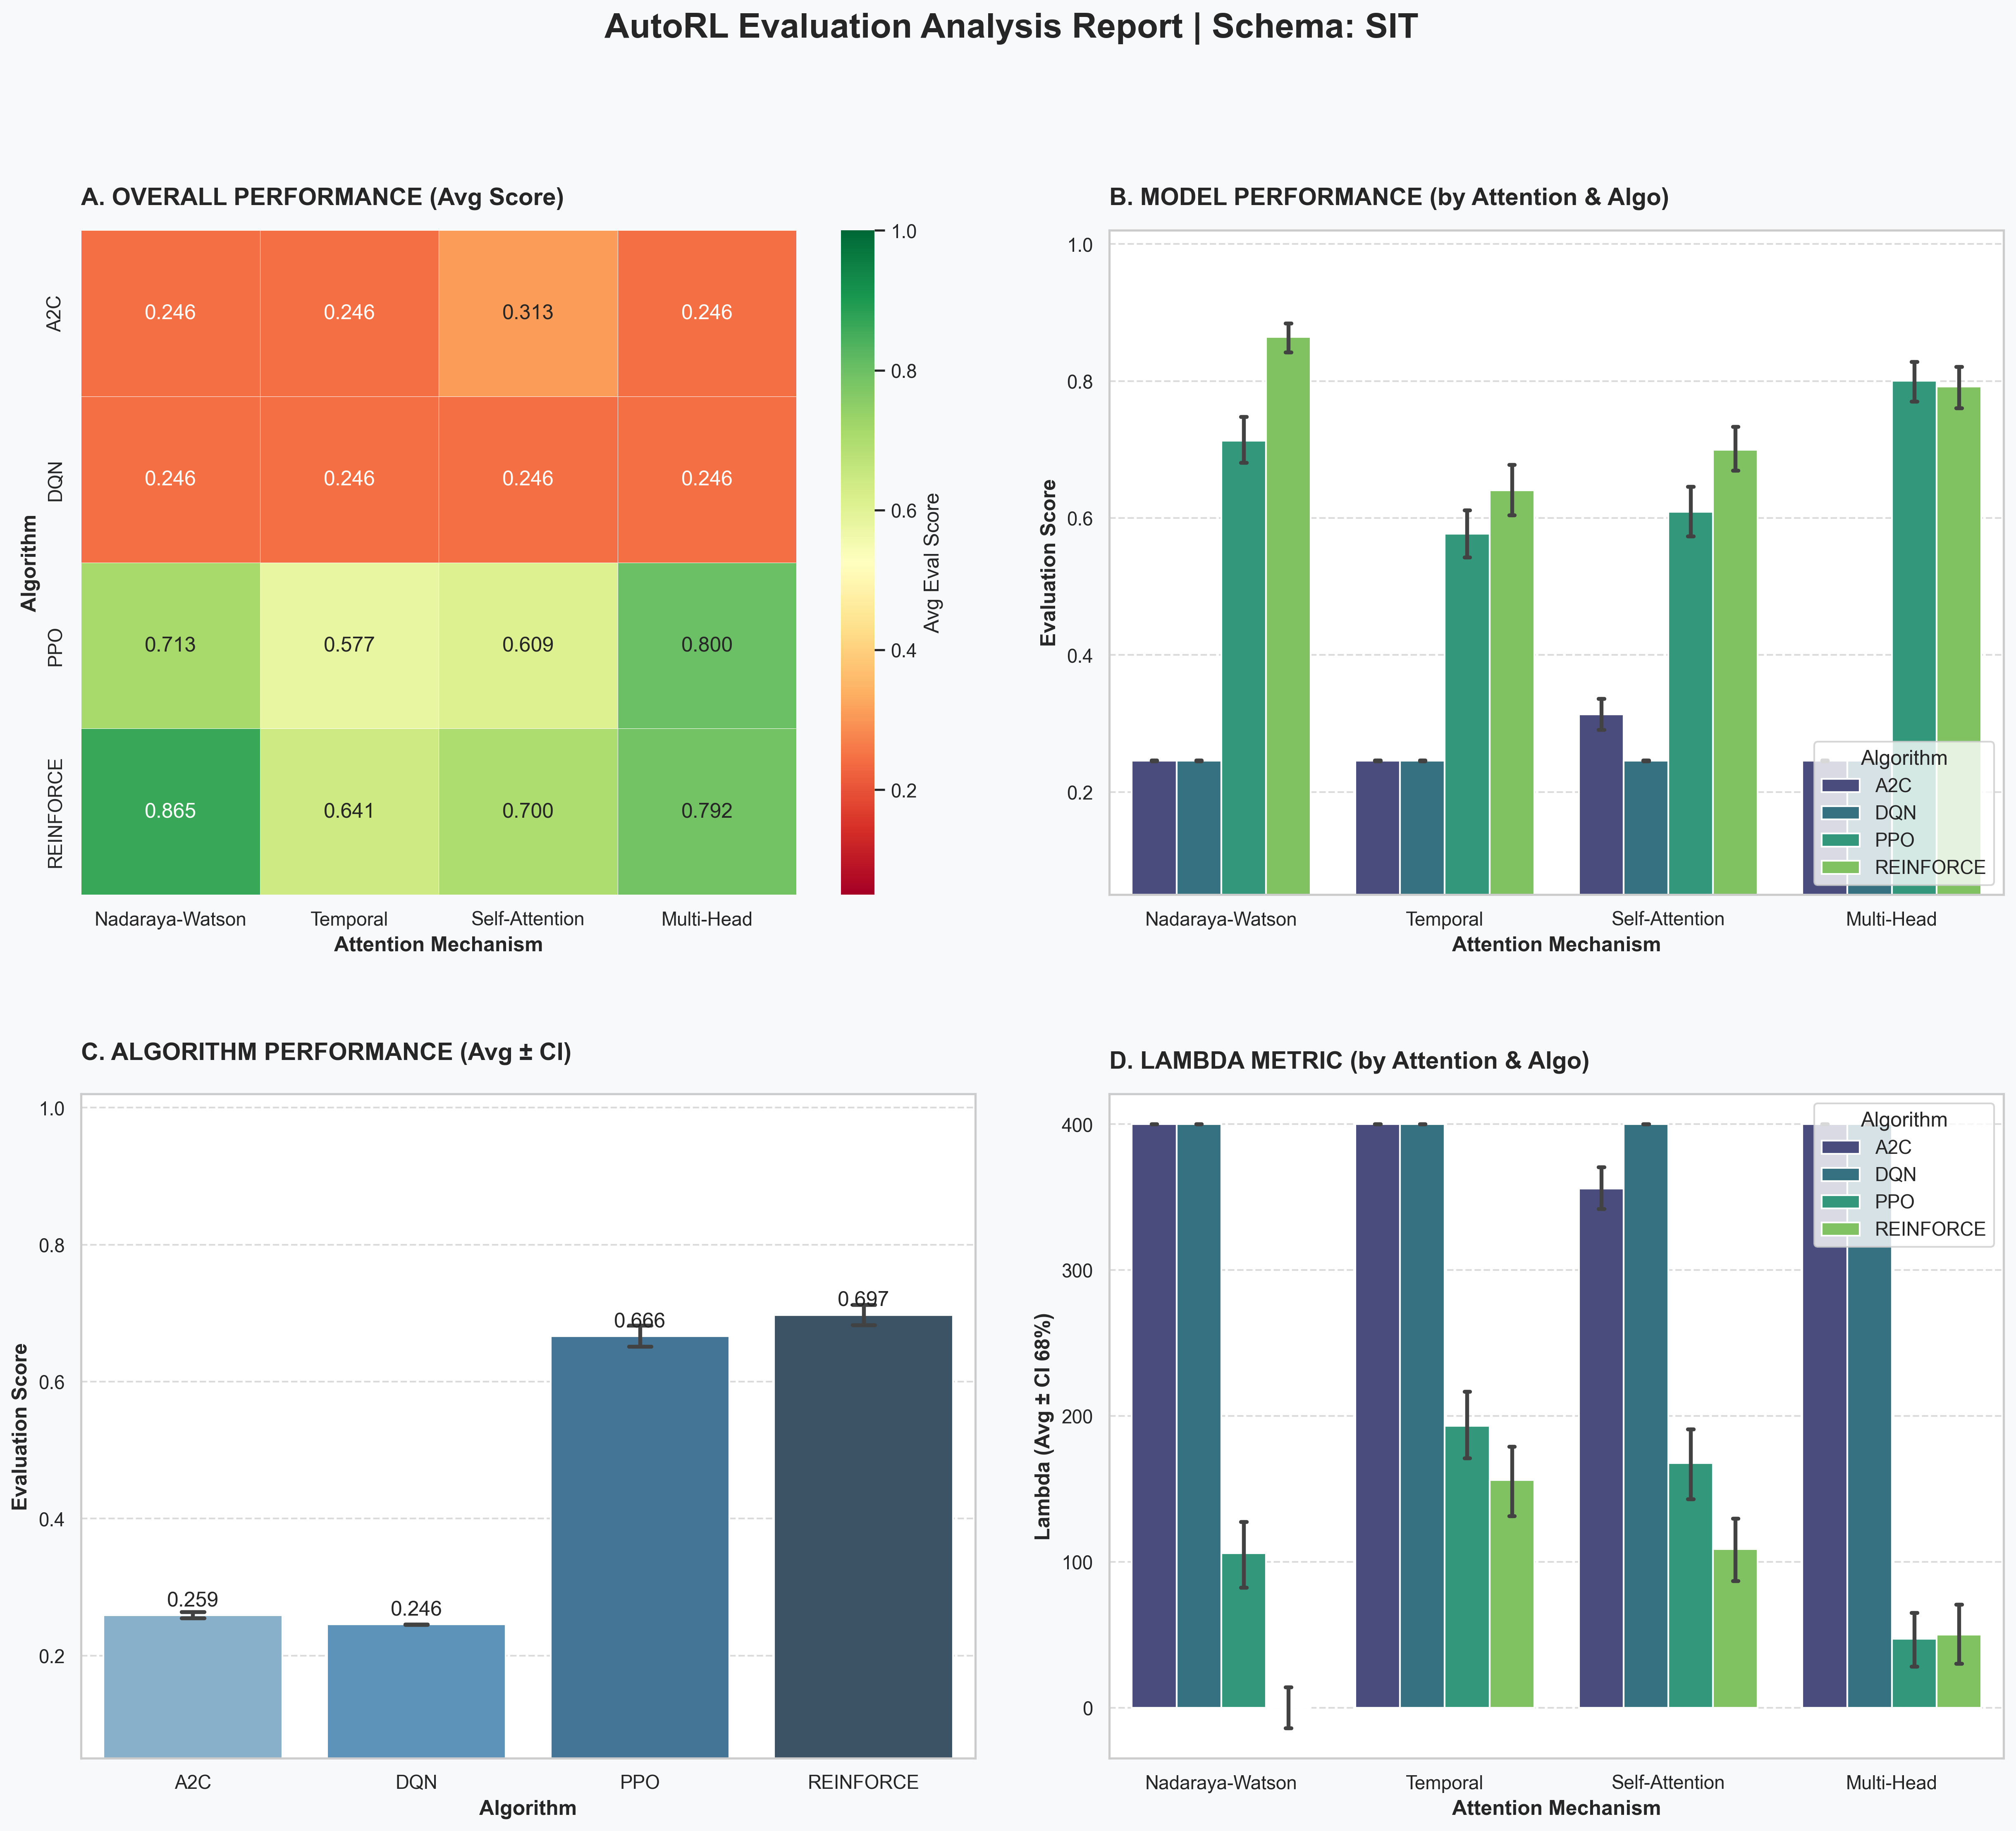
\includegraphics[width=\linewidth]{Analysis_Report_SIT.png}
		\caption{SIT analysis report.}
	\end{subfigure}
	\caption{Overall analysis reports.}
	\label{fig:analysis_reports}
\end{figure}

\begin{figure}[t]
	\centering
	\begin{subfigure}[t]{\textwidth}
		\centering
		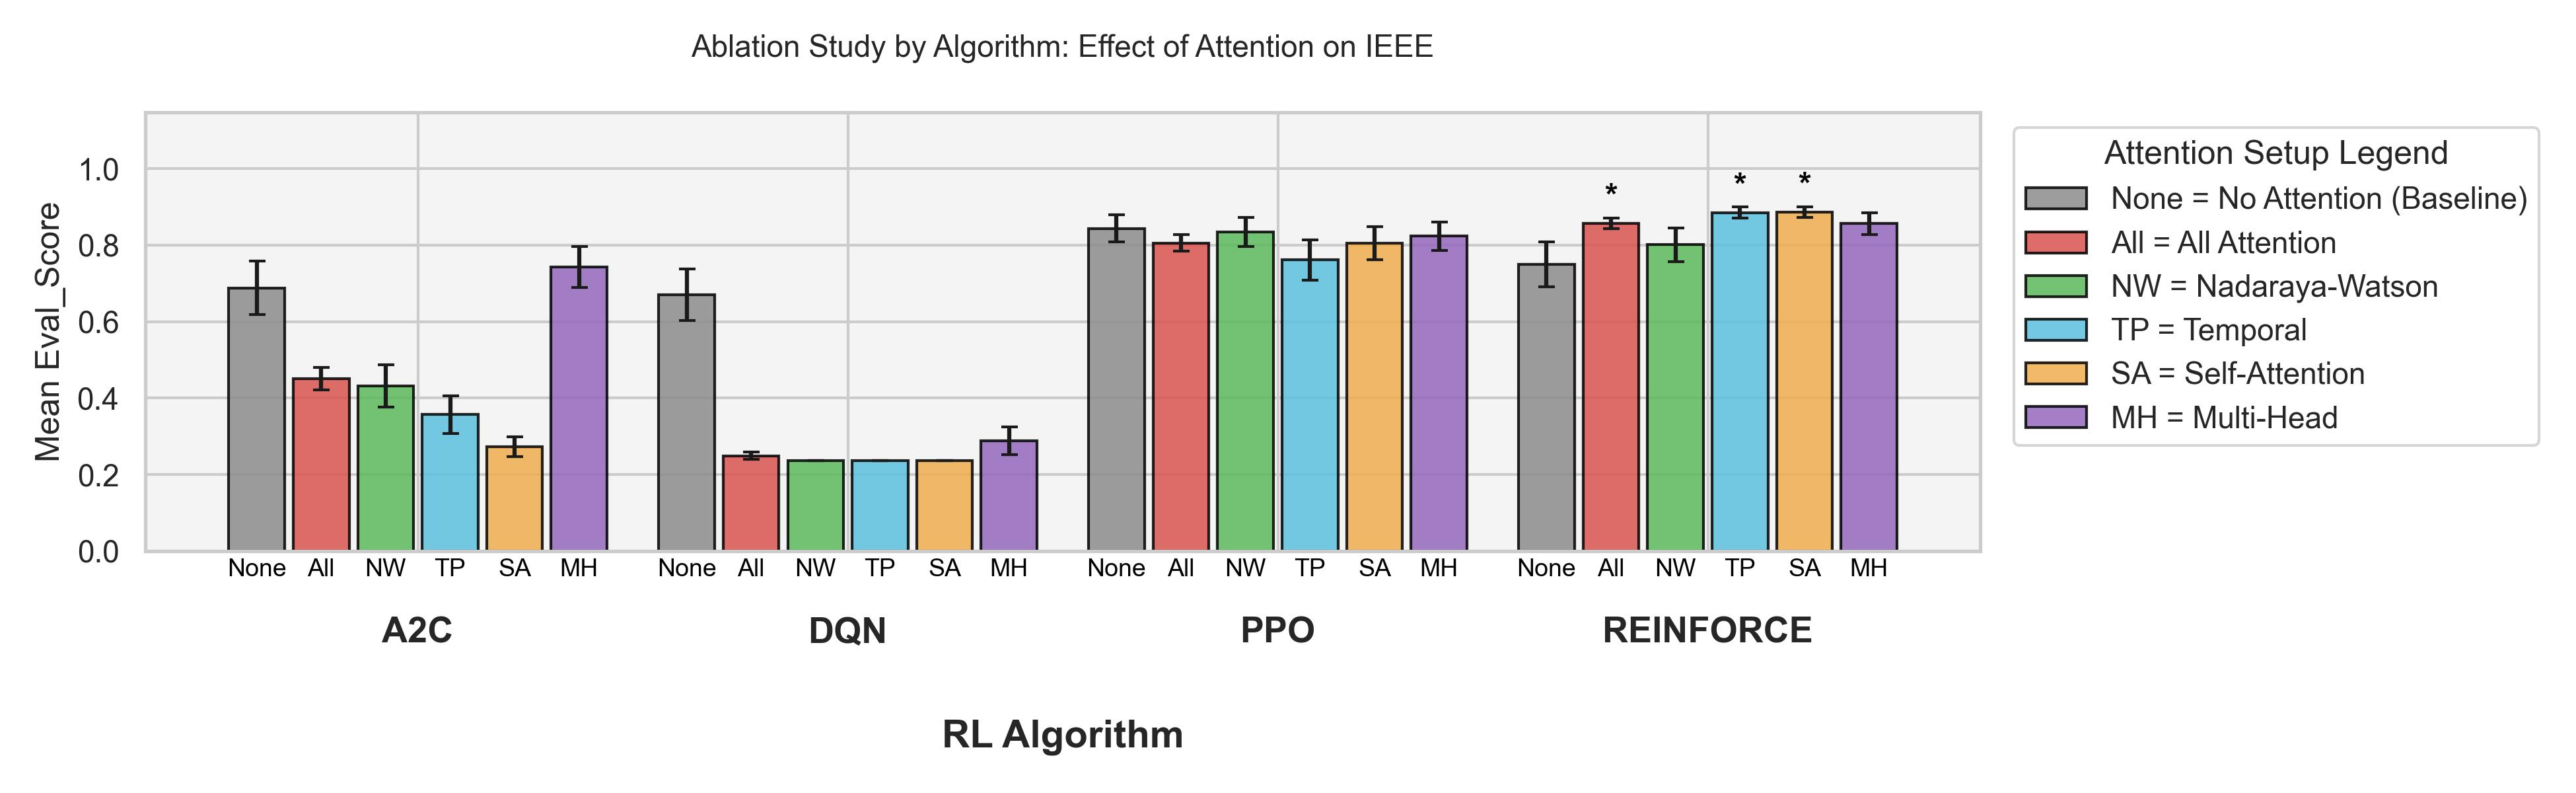
\includegraphics[width=\linewidth]{Ablation_Study_Algo_IEEE.jpg}
		\caption{IEEE ablation by algorithm.}
	\end{subfigure}

	\begin{subfigure}[t]{\textwidth}
		\centering
		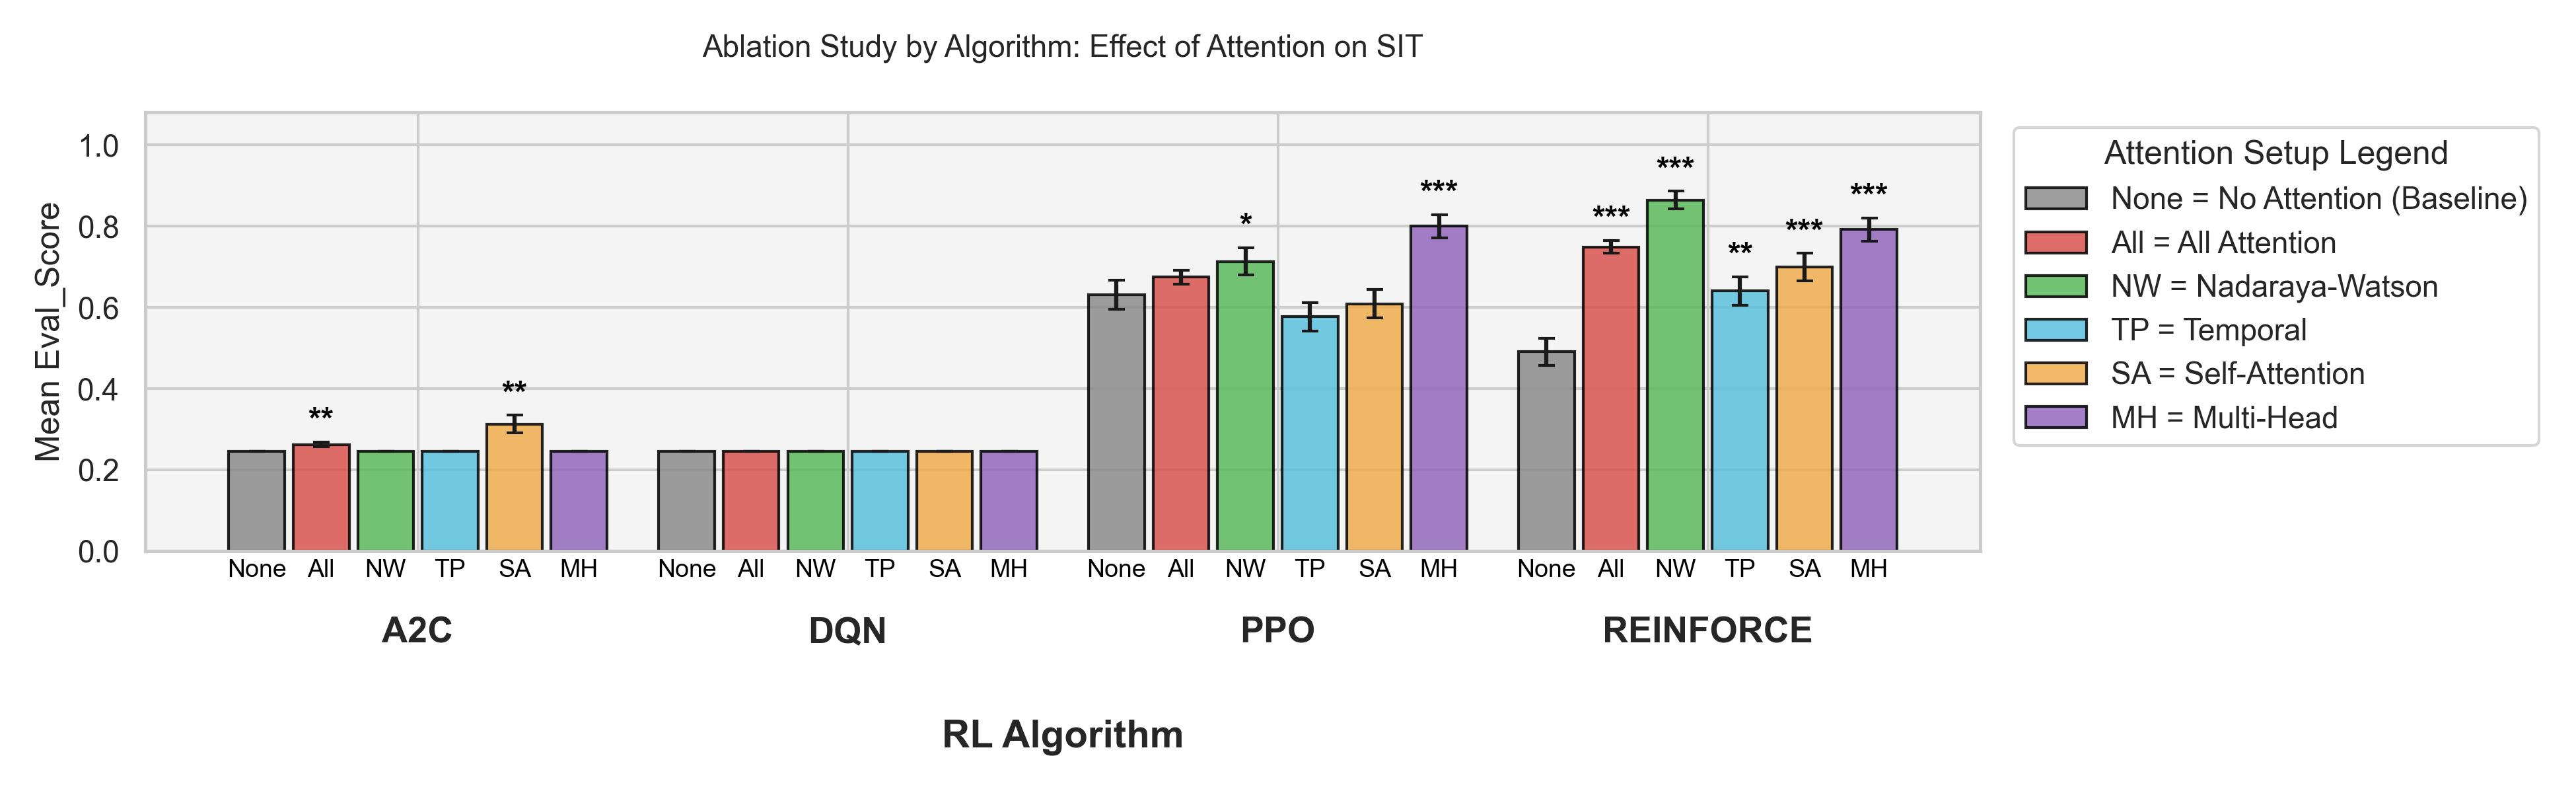
\includegraphics[width=\linewidth]{Ablation_Study_Algo_SIT.jpg}
		\caption{SIT ablation by algorithm.}
	\end{subfigure}
	\caption{Algorithm-level ablation summaries.}
	\label{fig:ablation_algo}
\end{figure}

\begin{figure}[t]
	\centering
	\begin{subfigure}[t]{0.9\textwidth}
		\centering
		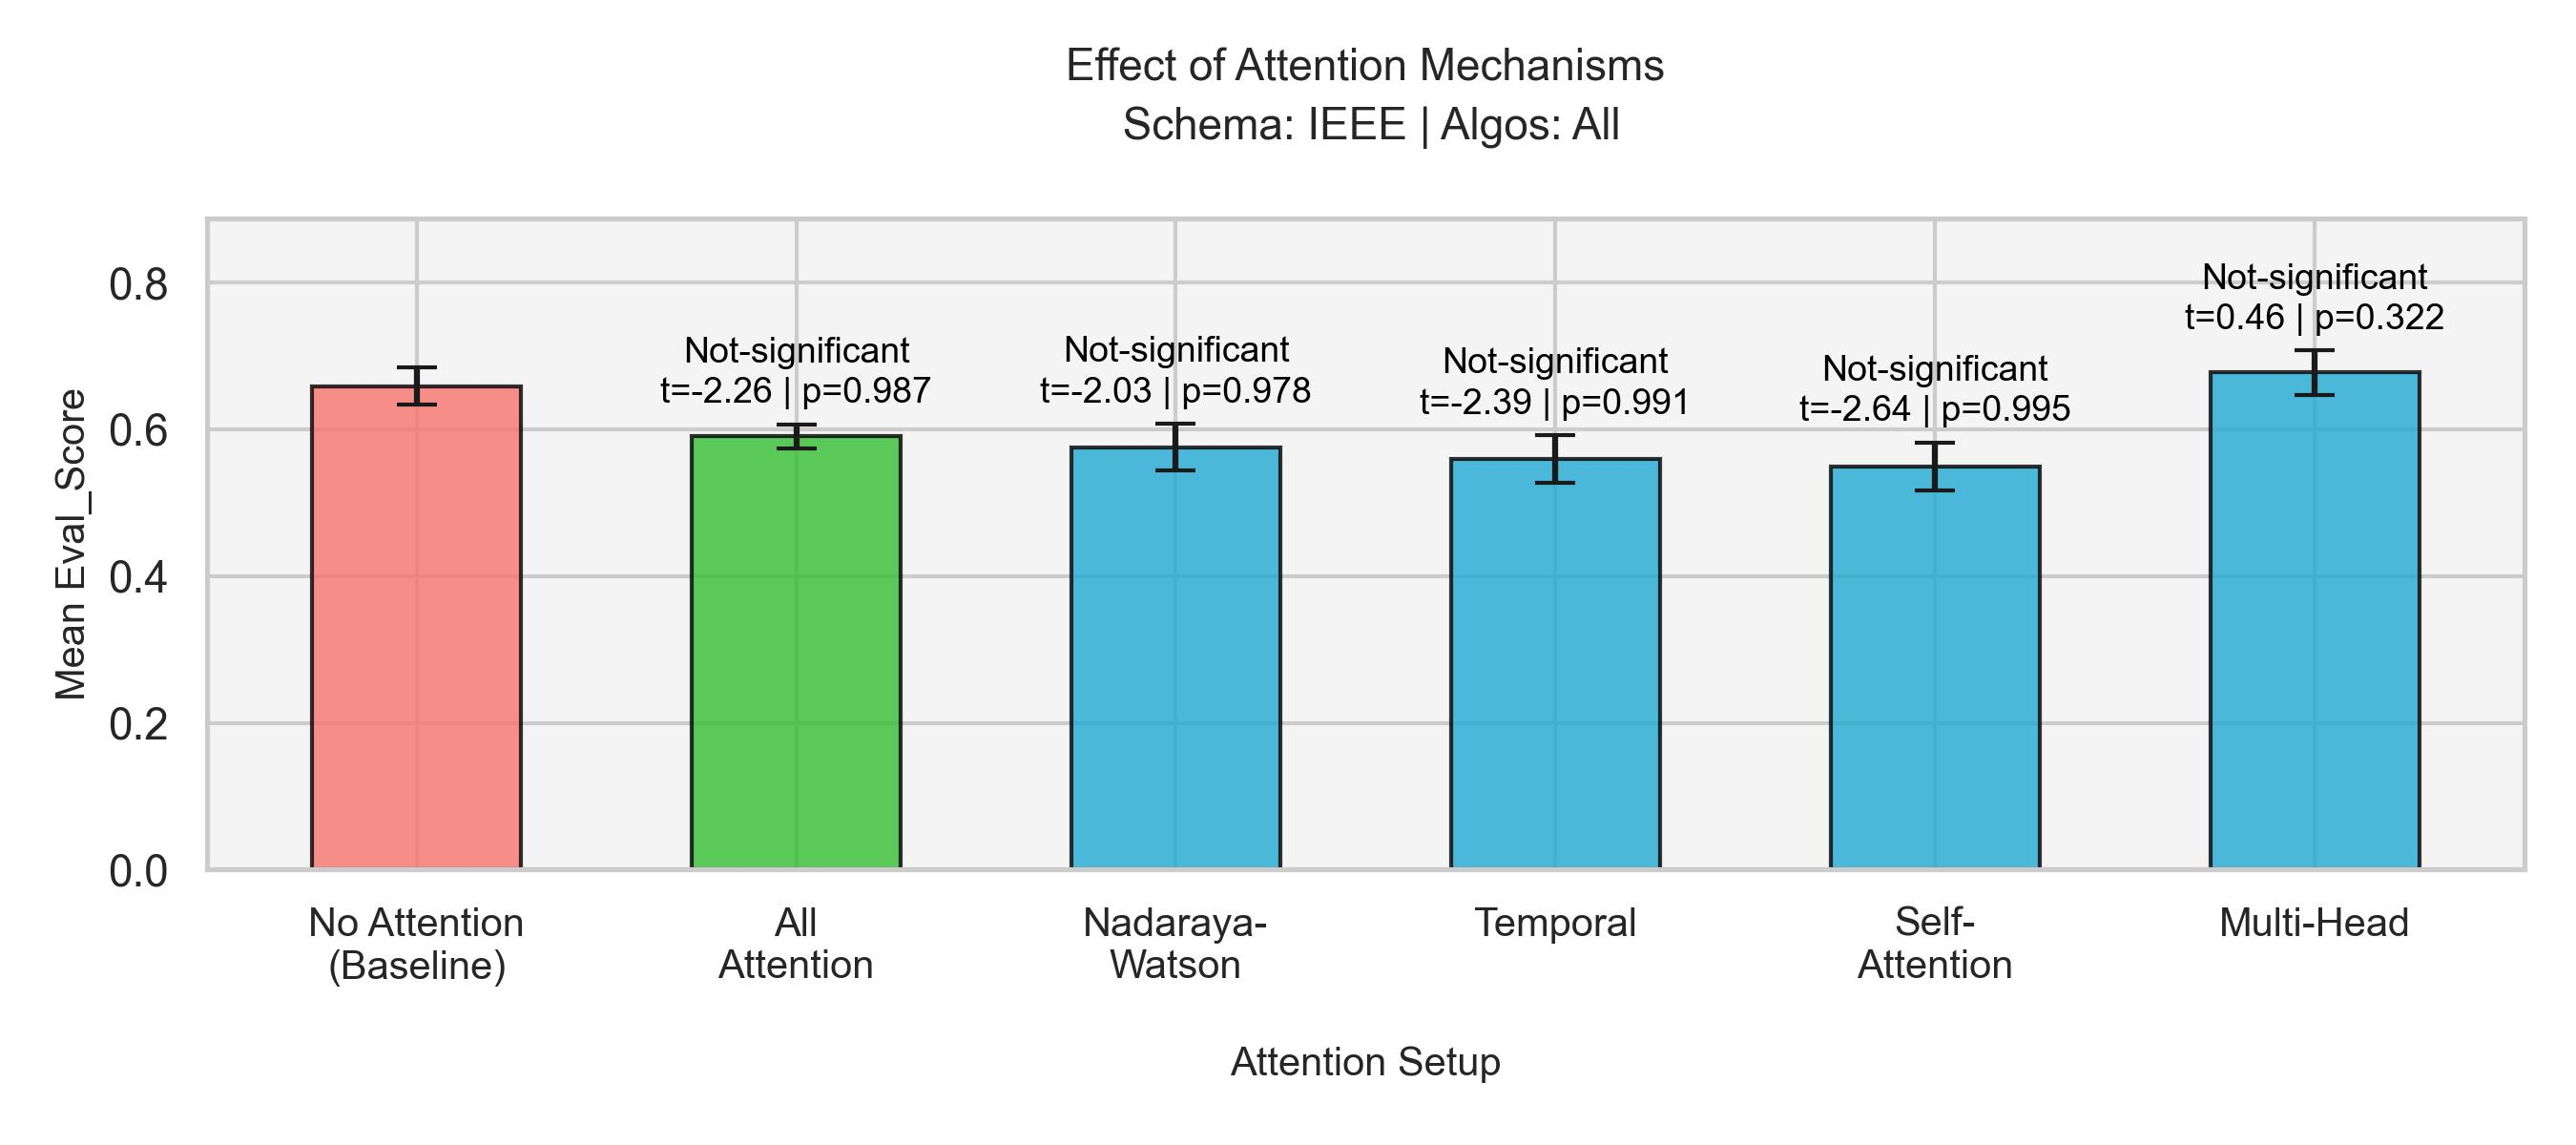
\includegraphics[width=\linewidth]{Ablation_Study_IEEE_All_Algos.jpg}
		\caption{IEEE: all algorithms pooled.}
	\end{subfigure}
	
	\begin{subfigure}[t]{0.9\textwidth}
		\centering
		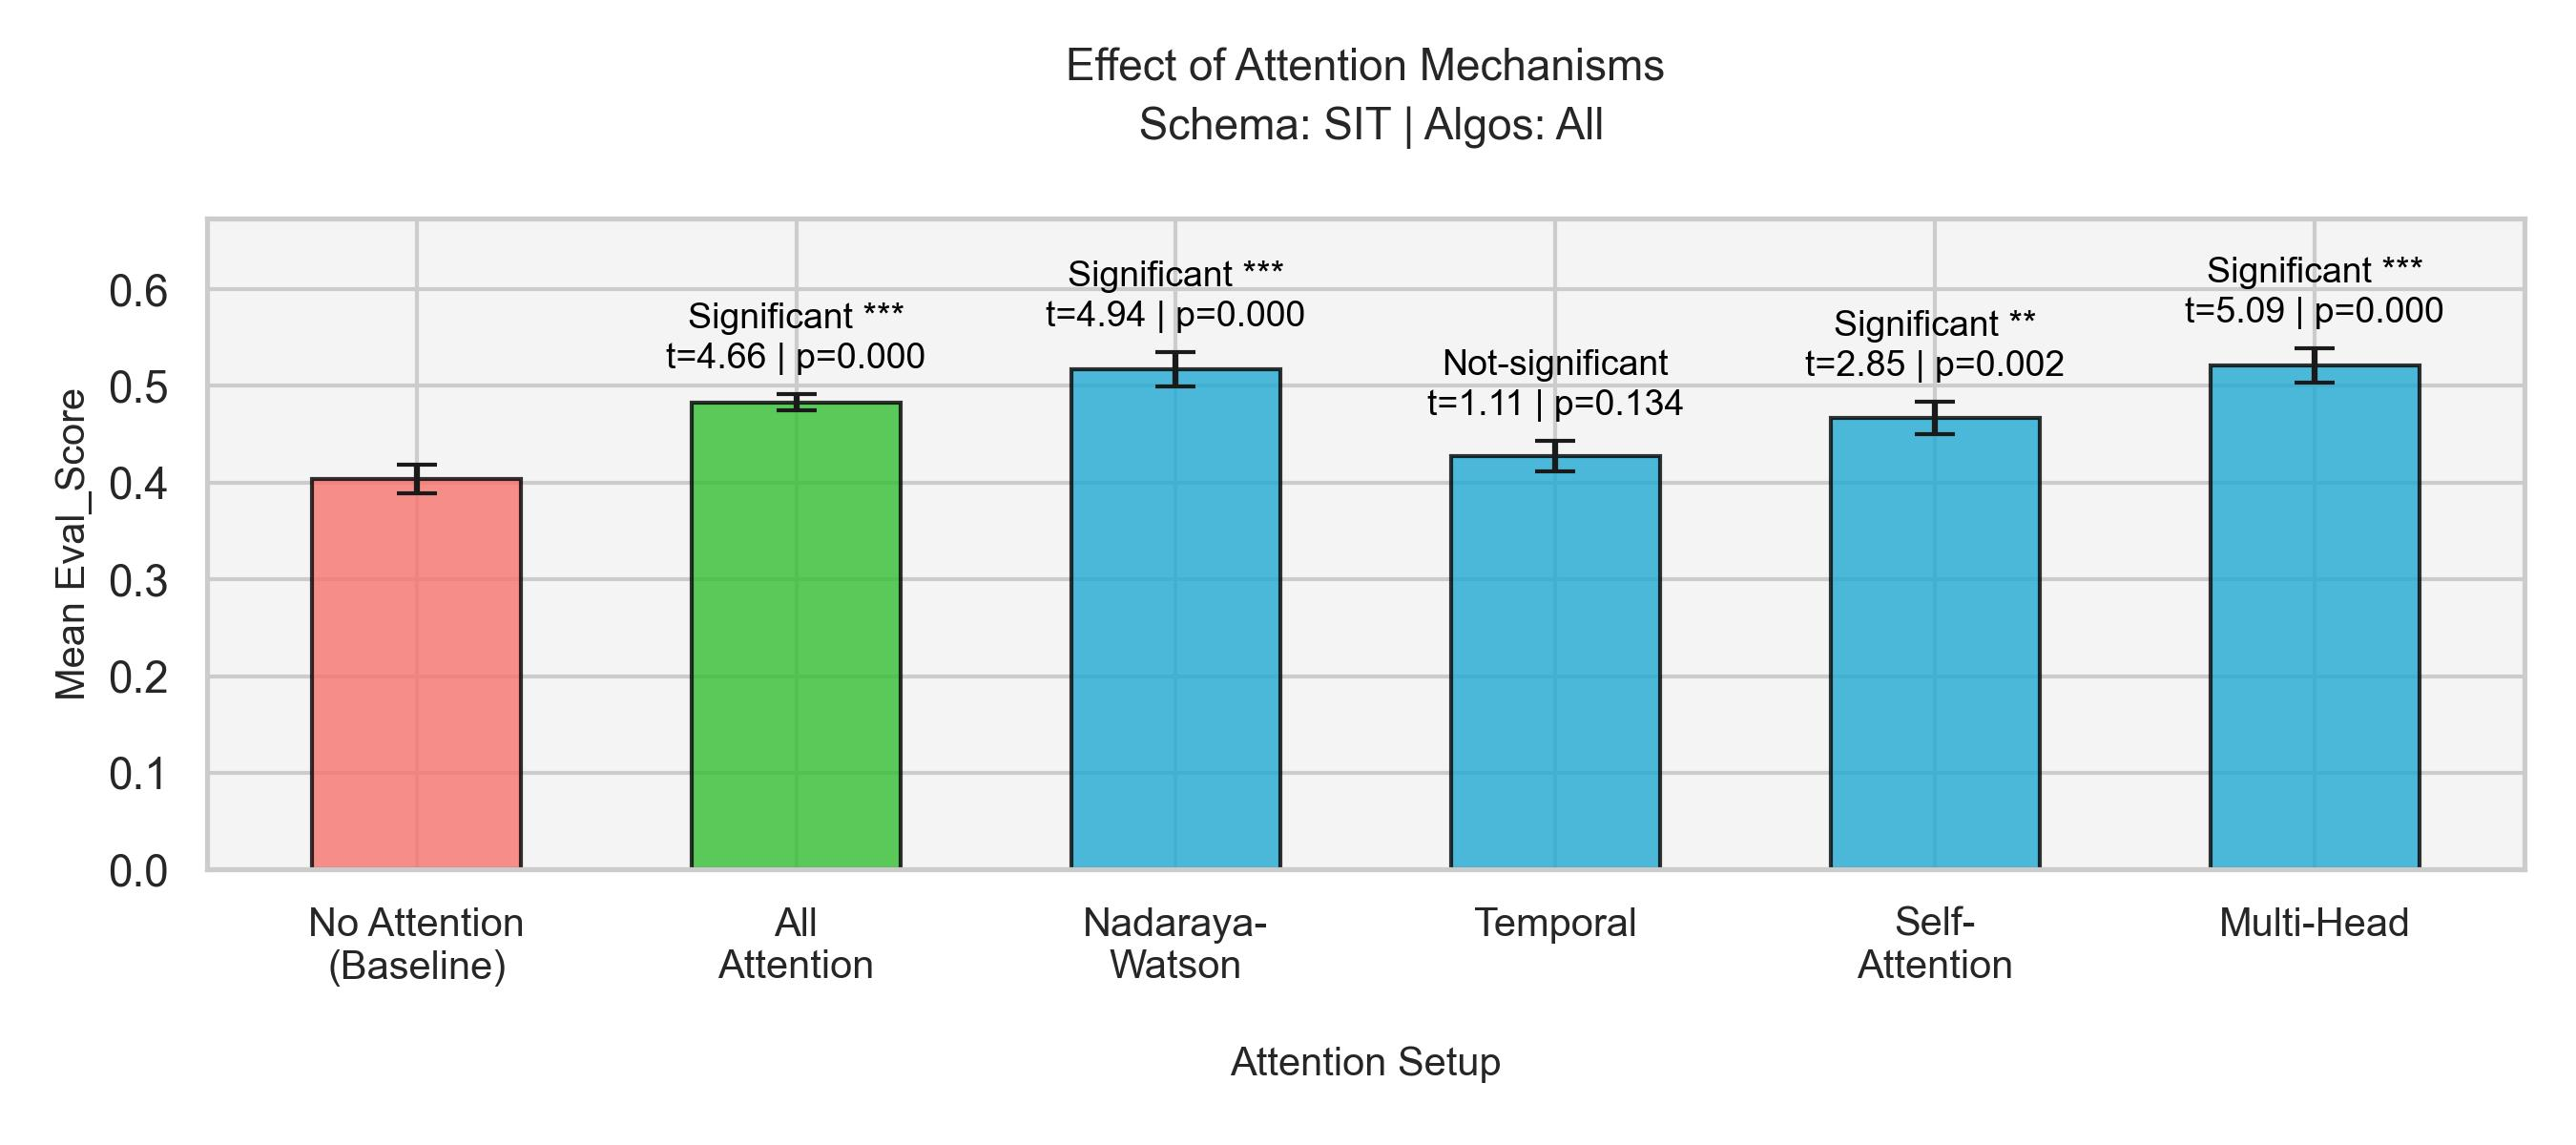
\includegraphics[width=\linewidth]{Ablation_Study_SIT_All_Algos.jpg}
		\caption{SIT: all algorithms pooled.}
	\end{subfigure}
	\caption{All-algorithm pooled ablation comparisons.}
	\label{fig:ablation_all}
\end{figure}

\begin{figure}[t]
	\centering
	\begin{subfigure}[t]{0.9\textwidth}
		\centering
		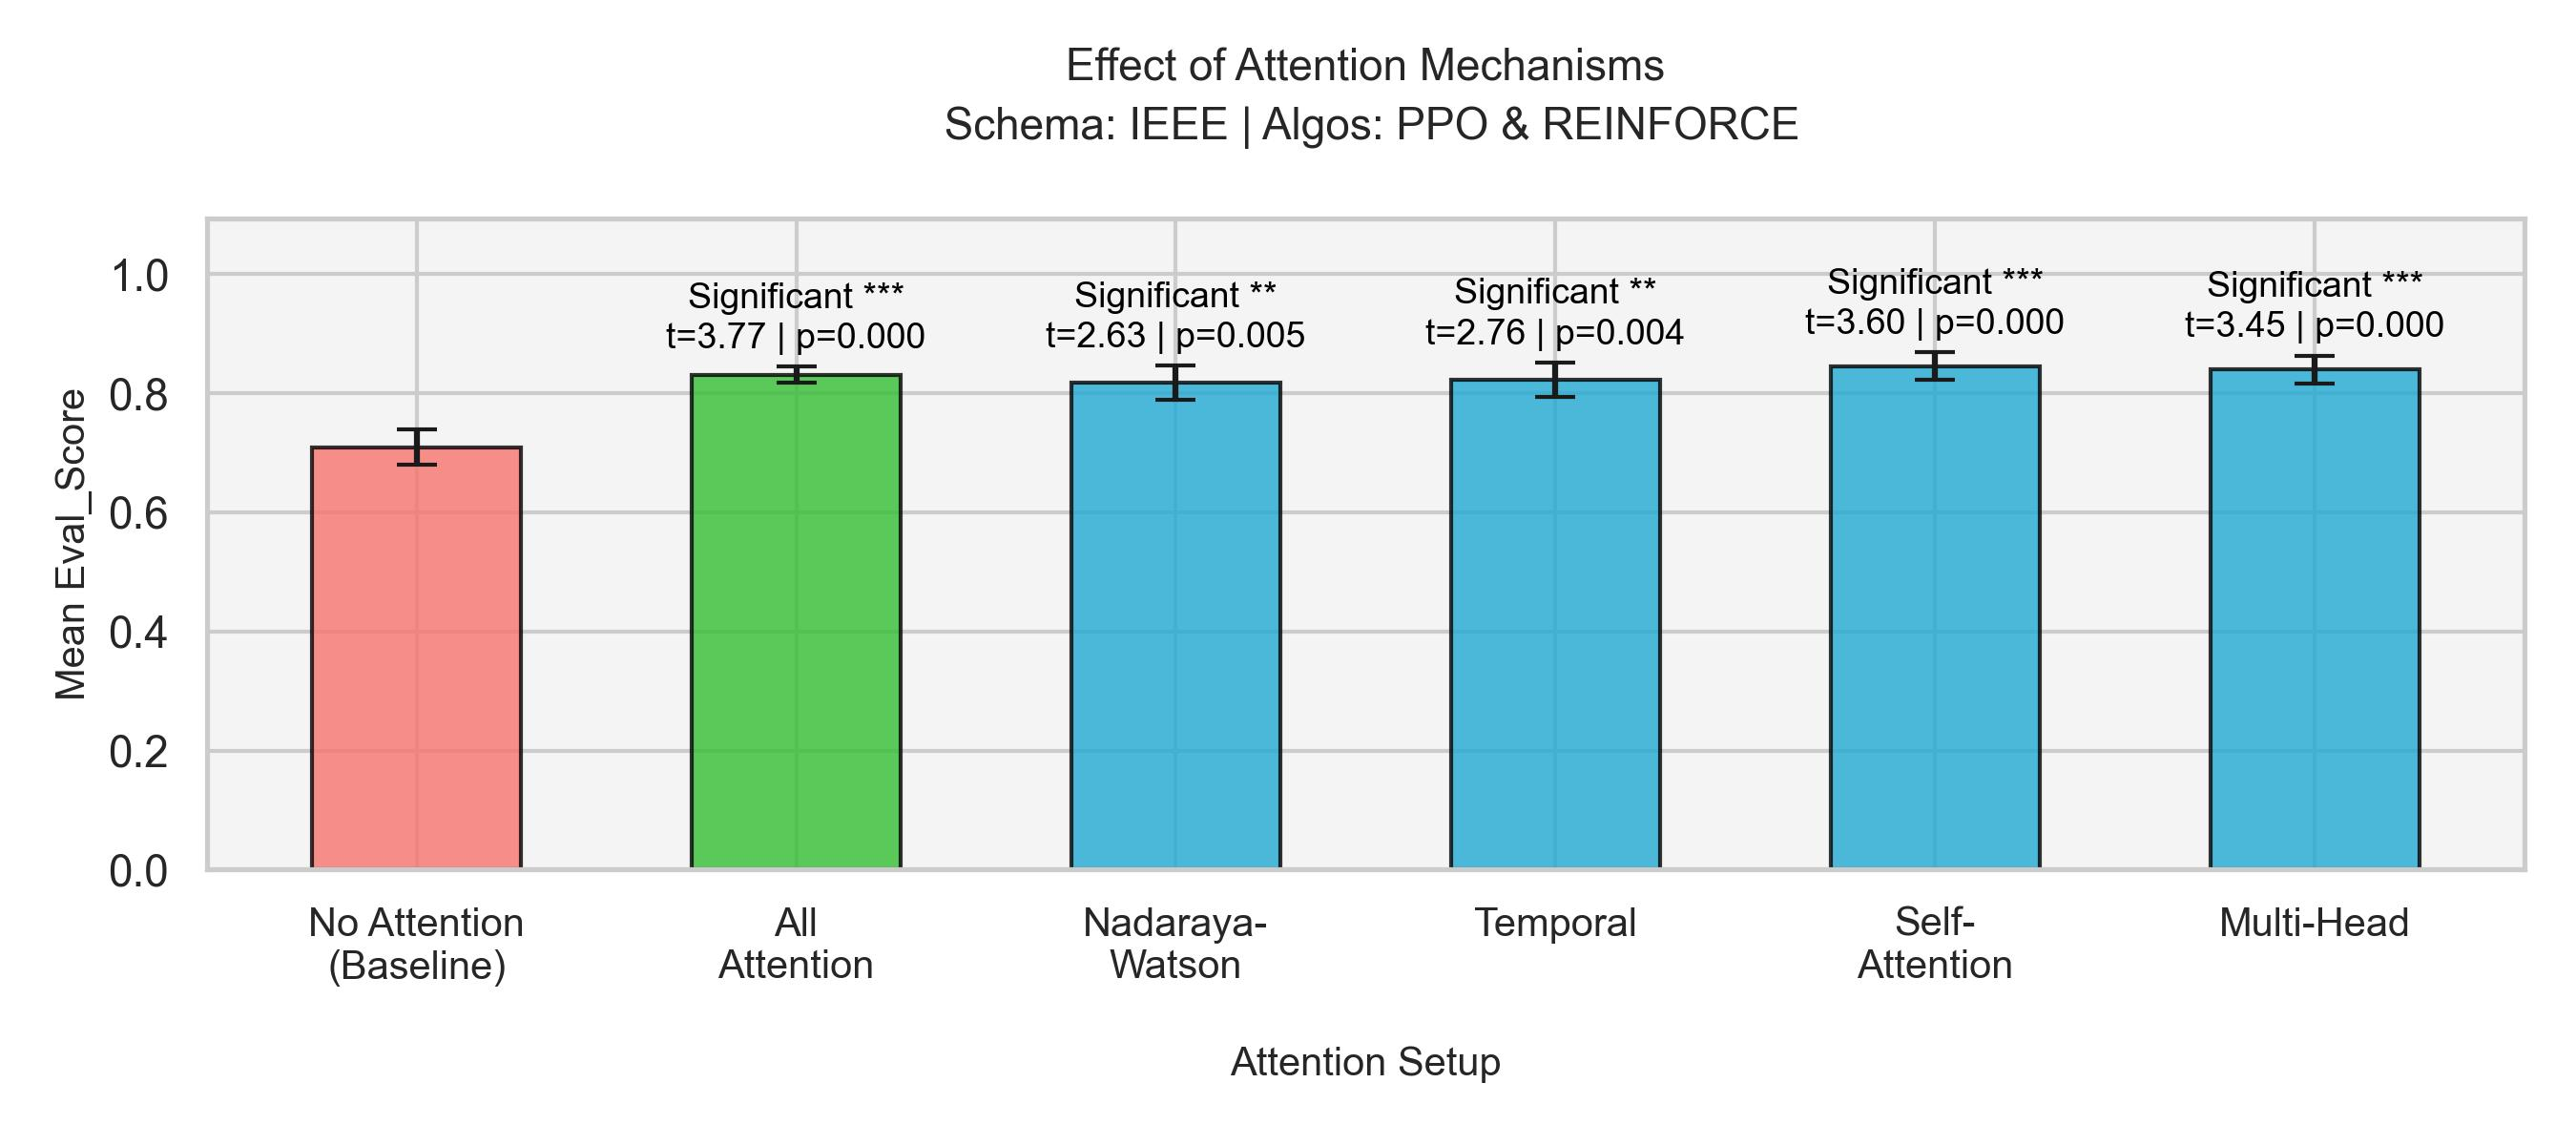
\includegraphics[width=\linewidth]{Ablation_Study_IEEE_PPO_REINFORCE.jpg}
		\caption{IEEE: PPO + \textsc{REINFORCE}.}
	\end{subfigure}
	
	\begin{subfigure}[t]{0.9\textwidth}
		\centering
		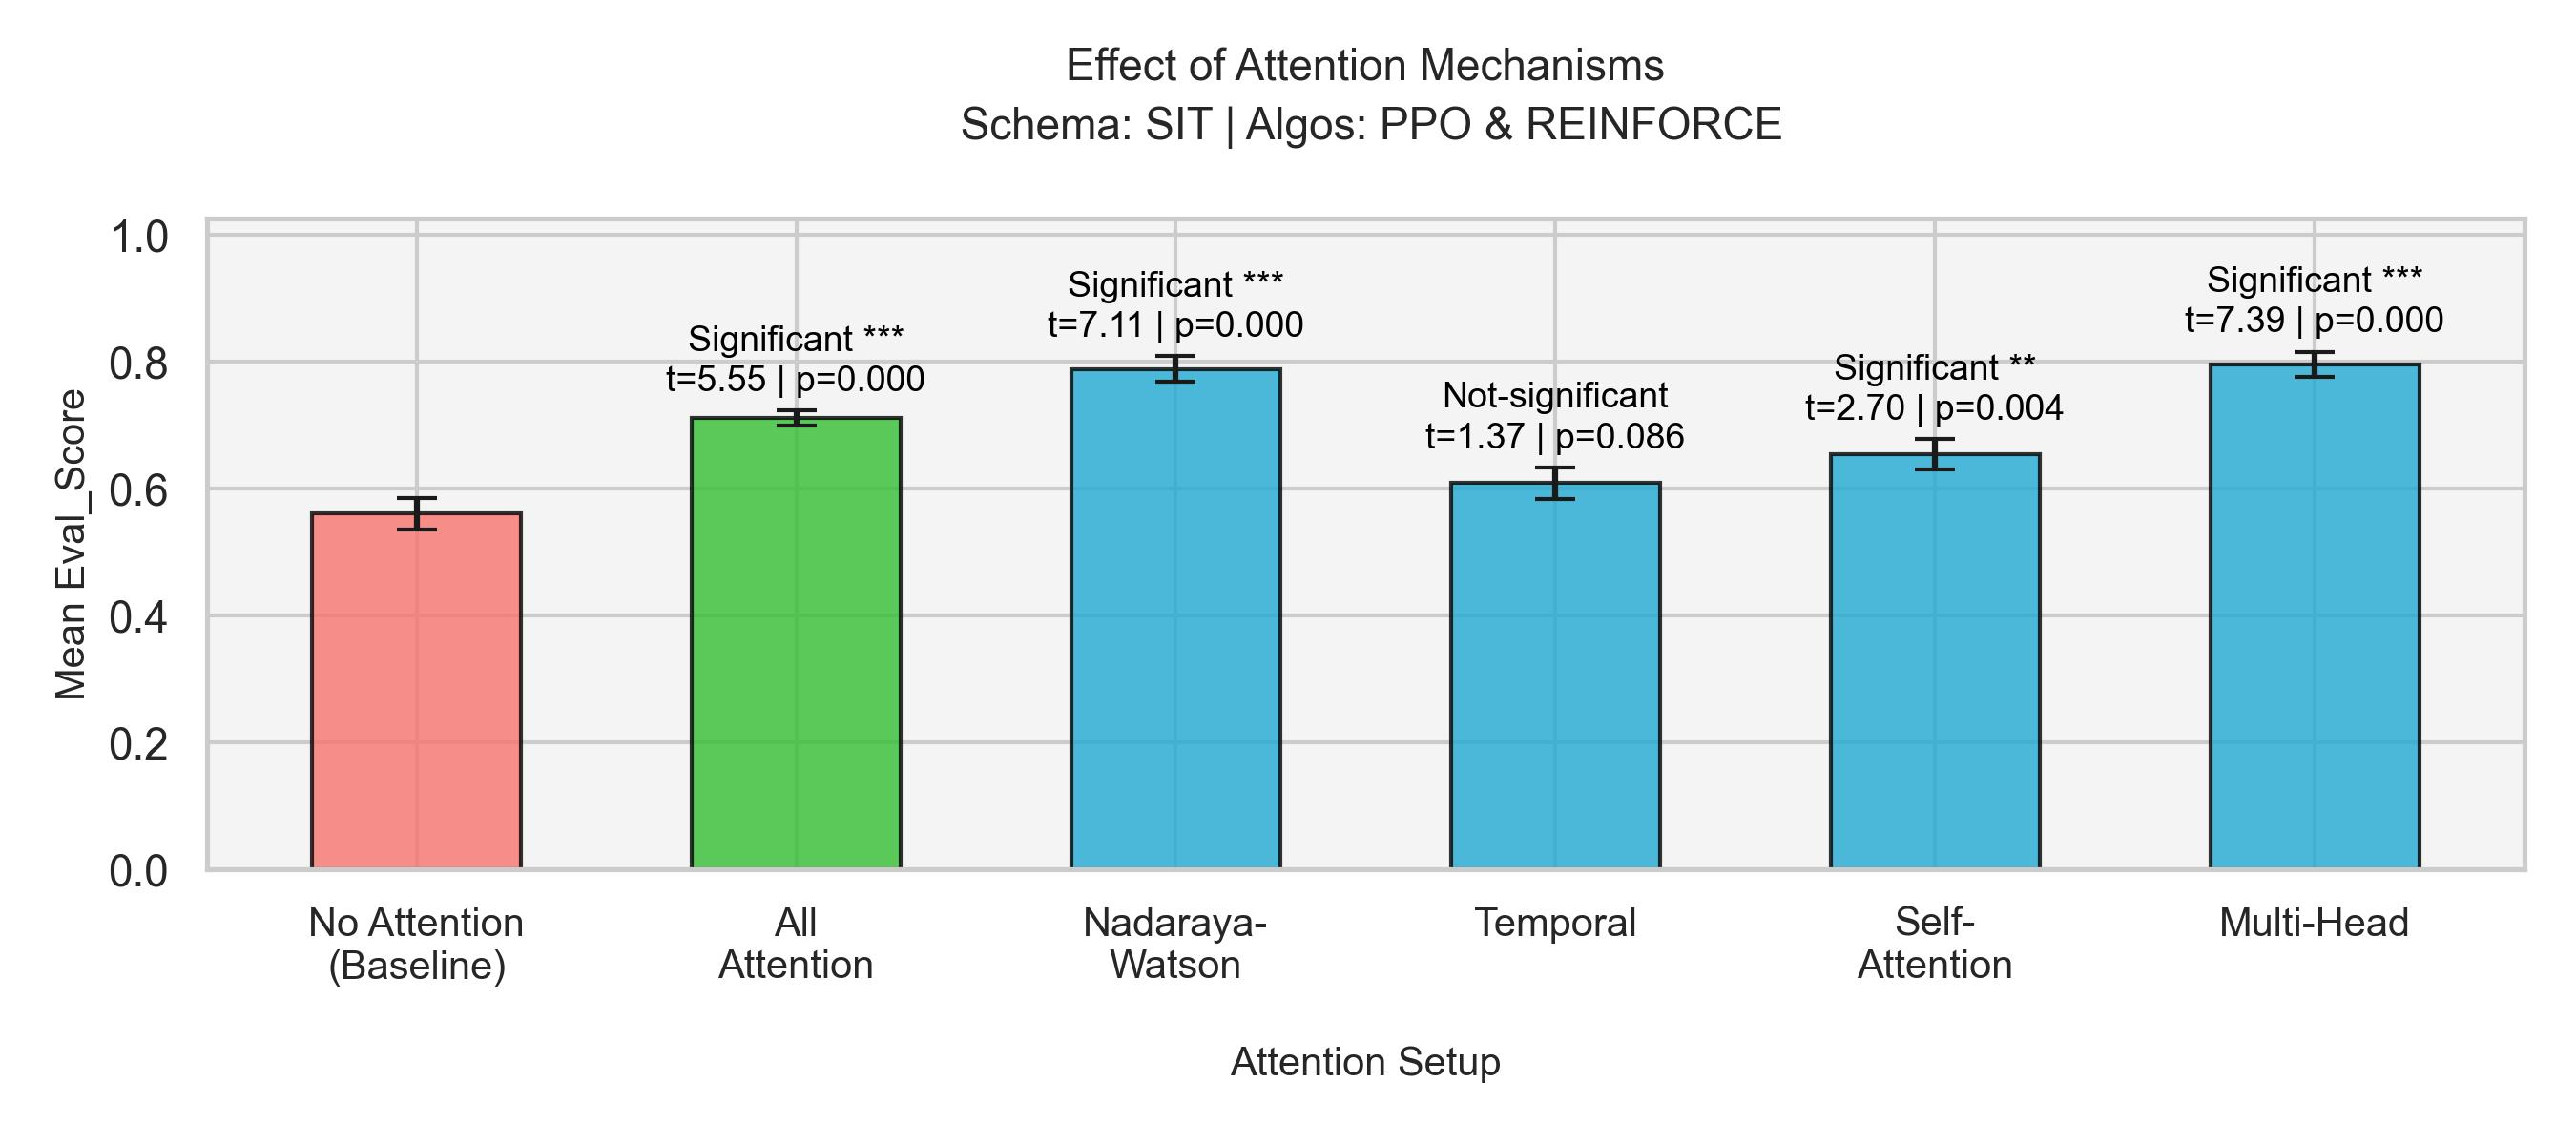
\includegraphics[width=\linewidth]{Ablation_Study_SIT_PPO_REINFORCE.jpg}
		\caption{SIT: PPO + \textsc{REINFORCE}.}
	\end{subfigure}
	\caption{Ablation comparisons focused on PPO and \textsc{REINFORCE}.}
	\label{fig:ablation_ppo_rf}
\end{figure}

\subsection{Schema portability and attention sensitivity}
While the reward structure and state-transition dynamics remain identical across schemas, feature complexity varies significantly. In SIT, non-parametric spatial attention (Nadaraya--Watson) provides maximum gain for Monte Carlo optimization (\textbf{0.8646}). In IEEE, high-dimensional temporal features require projection-based transformers (Self-Attention and Multi-Head), pushing \textsc{REINFORCE} scores to \textbf{0.8860}.

\subsection{Model sizes}
Serialized policy sizes remain compact across both schemas (Table~\ref{tab:model_size_summary}), making them suitable for embedded edge deployment.

\begin{table}[htbp]
\centering
\caption{Average serialized policy size (kB), averaged over models within each schema.}
\label{tab:model_size_summary}
\begin{tabular}{l r r}
\toprule
	\textbf{Algorithm} & \textbf{SIT avg. (kB)} & \textbf{IEEE avg. (kB)}\\
	\midrule
	A2C & 293.55 & 292.54\\
	DQN & 419.73 & 417.72\\
	PPO & 169.90 & 169.38\\
	\textbf{REINFORCE} & \textbf{169.47} & \textbf{168.95}\\
\bottomrule
\end{tabular}
\end{table}

% =================================================================
% DISCUSSION SECTION
% =================================================================

\section{Discussion}
\label{sec:discussion}

\subsection{Taxonomy of Evaluated RL Paradigms and Dynamic Representation Interactions}

To explain the performance divergence between algorithm families, we organize the evaluated algorithms into an architectural taxonomy (Figure~\ref{fig:rl_taxonomy_tree}) and map their functional interaction with dynamic attention feature layers (Figure~\ref{fig:rl_attention_interaction}).

% -----------------------------------------------------------------
% FIGURE 1: TAXONOMY TREE DIAGRAM (TikZ)
% -----------------------------------------------------------------
\begin{figure}[htbp]
\centering
\resizebox{\linewidth}{!}{%
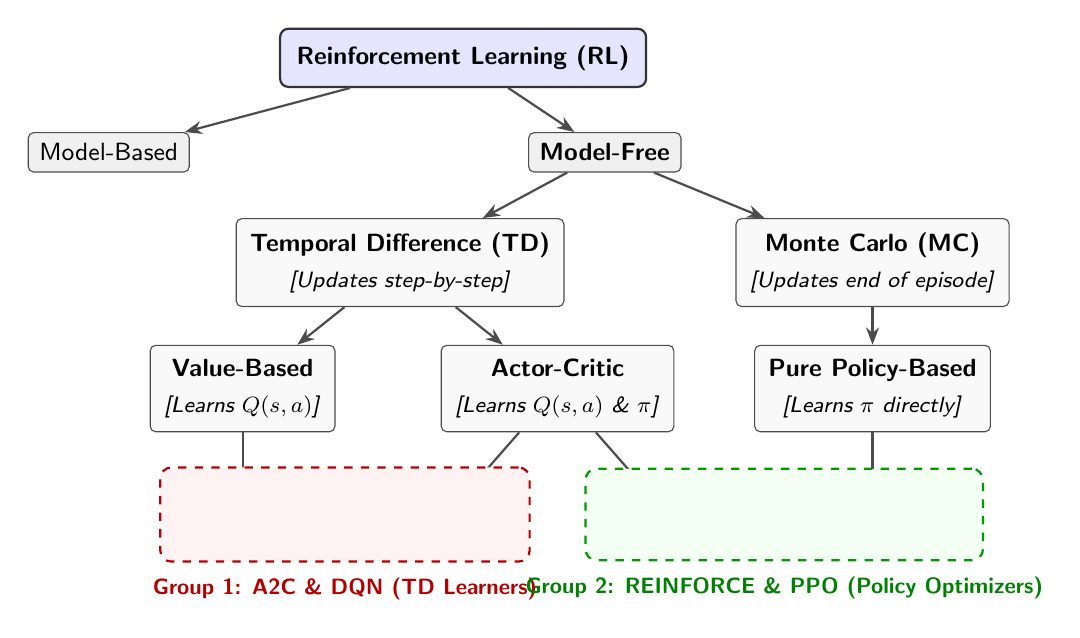
\begin{tikzpicture}[
    font=\sffamily\small,
    root/.style={rectangle, draw=black!80, fill=blue!10, thick, rounded corners=3pt, align=center, inner sep=6pt, font=\sffamily\bfseries\small},
    level1/.style={rectangle, draw=black!70, fill=gray!12, rounded corners=2pt, align=center, inner sep=4pt},
    level2/.style={rectangle, draw=black!70, fill=gray!5, rounded corners=2pt, align=center, inner sep=5pt},
    algo/.style={rectangle, draw=blue!80!black, fill=blue!10, thick, rounded corners=3pt, align=center, inner sep=5pt, font=\sffamily\bfseries\small, minimum width=1.5cm},
    group1/.style={rectangle, draw=red!70!black, fill=red!5, dashed, thick, rounded corners=4pt, inner sep=8pt},
    group2/.style={rectangle, draw=green!60!black, fill=green!5, dashed, thick, rounded corners=4pt, inner sep=8pt},
    edge_style/.style={draw=black!70, -{Stealth[length=2.2mm]}, thick}
]

% Level 0: Root
\node[root] (rl) at (0, 0) {Reinforcement Learning (RL)};

% Level 1: Model-Based / Model-Free
\node[level1] (mb) at (-4.5, -1.2) {Model-Based};
\node[level1] (mf) at (1.8, -1.2) {\textbf{Model-Free}};

% Level 2: TD / MC
\node[level2] (td) at (-0.8, -2.6) {\textbf{Temporal Difference (TD)}\\[2pt]\textit{\footnotesize [Updates step-by-step]}};
\node[level2] (mc) at (5.2, -2.6) {\textbf{Monte Carlo (MC)}\\[2pt]\textit{\footnotesize [Updates end of episode]}};

% Level 3: Paradigms
\node[level2] (vb) at (-2.8, -4.2) {\textbf{Value-Based}\\[2pt]\textit{\footnotesize [Learns $Q(s,a)$]}};
\node[level2] (ac) at (1.2, -4.2) {\textbf{Actor-Critic}\\[2pt]\textit{\footnotesize [Learns $Q(s,a)$ \& $\pi$]}};
\node[level2] (pb) at (5.2, -4.2) {\textbf{Pure Policy-Based}\\[2pt]\textit{\footnotesize [Learns $\pi$ directly]}};

% Level 4: Algorithm Nodes
\node[algo] (dqn) at (-2.8, -5.8) {DQN};
\node[algo] (a2c) at (-0.2, -5.8) {A2C};
\node[algo] (ppo) at (2.6, -5.8) {PPO};
\node[algo] (rf) at (5.2, -5.8) {REINFORCE};

% Connections
\draw[edge_style] (rl) -- (mb);
\draw[edge_style] (rl) -- (mf);
\draw[edge_style] (mf) -- (td);
\draw[edge_style] (mf) -- (mc);
\draw[edge_style] (td) -- (vb);
\draw[edge_style] (td) -- (ac);
\draw[edge_style] (mc) -- (pb);
\draw[edge_style] (vb) -- (dqn);
\draw[edge_style] (ac) -- (a2c);
\draw[edge_style] (ac) -- (ppo);
\draw[edge_style] (pb) -- (rf);

% Group Boxes
\node[group1, fit=(dqn) (a2c), label={[font=\sffamily\bfseries\footnotesize, text=red!70!black, yshift=-2pt]below:Group 1: A2C \& DQN (TD Learners)}] (g1) {};
\node[group2, fit=(ppo) (rf), label={[font=\sffamily\bfseries\footnotesize, text=green!50!black, yshift=-2pt]below:Group 2: REINFORCE \& PPO (Policy Optimizers)}] (g2) {};

\end{tikzpicture}%
}
\caption{Taxonomy tree of reinforcement learning algorithm families evaluated in this study.}
\label{fig:rl_taxonomy_tree}
\end{figure}

% -----------------------------------------------------------------
% FIGURE 2: DYNAMIC FEATURE INTERACTION DIAGRAM (TikZ)
% -----------------------------------------------------------------
\begin{figure}[htbp]
\centering
\resizebox{\linewidth}{!}{%
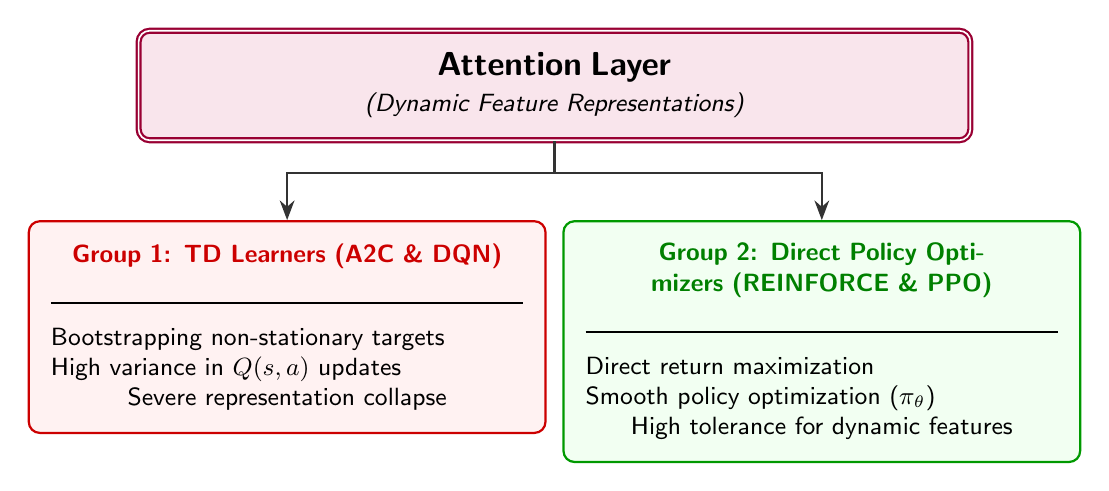
\begin{tikzpicture}[
    font=\sffamily\small,
    attn/.style={rectangle, draw=purple!80!black, fill=purple!10, double, thick, rounded corners=4pt, align=center, inner sep=8pt, text width=10cm},
    g1_box/.style={rectangle, draw=red!80!black, fill=red!5, thick, rounded corners=4pt, align=center, inner sep=8pt, text width=6cm},
    g2_box/.style={rectangle, draw=green!60!black, fill=green!5, thick, rounded corners=4pt, align=center, inner sep=8pt, text width=6cm},
    arrow/.style={draw=black!80, -{Stealth[length=2.5mm]}, thick}
]

% Top Attention Layer
\node[attn] (attn_layer) {\textbf{\large Attention Layer}\\[2pt]\textit{(Dynamic Feature Representations)}};

% Group 1 Box (Left)
\node[g1_box, below left=1.0cm and 0.1cm of attn_layer.south] (g1) {
    \textbf{\textcolor{red!80!black}{Group 1: TD Learners (A2C \& DQN)}}\\[4pt]
    \rule{\linewidth}{0.4pt}\\[4pt]
    \raggedright
    Bootstrapping non-stationary targets\\
    High variance in $Q(s,a)$ updates\\
    Severe representation collapse
};

% Group 2 Box (Right)
\node[g2_box, below right=1.0cm and 0.1cm of attn_layer.south] (g2) {
    \textbf{\textcolor{green!50!black}{Group 2: Direct Policy Optimizers (REINFORCE \& PPO)}}\\[4pt]
    \rule{\linewidth}{0.4pt}\\[4pt]
    \raggedright
    Direct return maximization\\
    Smooth policy optimization ($\pi_\theta$)\\
    High tolerance for dynamic features
};

% Connections
\draw[arrow] (attn_layer.south) -- ++(0,-0.4) -| (g1.north);
\draw[arrow] (attn_layer.south) -- ++(0,-0.4) -| (g2.north);

\end{tikzpicture}%
}
\caption{Interaction model between dynamic attention layers and the two RL algorithmic taxonomy groups.}
\label{fig:rl_attention_interaction}
\end{figure}

\subsection{Theoretical Justification via Algorithmic Taxonomy}
The empirical split between \textbf{Group 1} (TD Learners) and \textbf{Group 2} (Direct Policy Optimizers) stems from how update mechanisms handle non-stationary state feature projections (Figure~\ref{fig:rl_attention_interaction}):

\begin{enumerate}
	\item \textbf{Group 1: TD Learners (\textsc{DQN} \& \textsc{A2C}):} These algorithms rely on Temporal Difference bootstrapping to update state-action value estimates $Q(s,a)$ or state values $V(s)$. When dynamic attention layers are placed upstream of the value networks, the state representation shifts during training, introducing non-stationarity into the bootstrapped Bellman target $Y_t^{\text{TD}}$. This instability makes $Q$-value estimates unreliable, explaining why \textsc{DQN} exhibits a substantial performance drop to the minimum score floor ($0.2360$) across attention setups.
    
	\item \textbf{Group 2: Direct Policy Optimizers (\textsc{REINFORCE} \& \textsc{PPO}):} These algorithms directly parameterize a policy $\pi_\theta(a|s)$ to maximize expected trajectory returns $J(\theta) = \mathbb{E}_{\pi_\theta}[R]$. Because Monte Carlo methods like \textsc{REINFORCE} utilize un-bootstrapped full-trajectory returns $G_t$, they are not affected by target non-stationarity in the same way. Dynamic attention layers act as adaptive filters that isolate degradation features from the high-dimensional sensor stream, simplifying the policy learning space (\textbf{0.8646} on SIT, \textbf{0.8860} on IEEE). \textsc{PPO} similarly benefits, as its clipped surrogate objective enforces trust-region bounds that manage policy updates when attention features shift.
\end{enumerate}

\subsection{Why \textsc{REINFORCE} may outperform \textsc{PPO} under attention}
In standard unaugmented RL setups, \textsc{PPO} is often a stronger baseline due to variance-reduction mechanisms and trust-region constraints ($0.6313$ vs. $0.4907$ in SIT; $0.7484$ vs. $0.6696$ in IEEE). 

However, \textsc{PPO}'s clipped objective restricts large policy updates. When paired with expressive feature extractors like attention, \textsc{REINFORCE}'s unconstrained policy updates allow it to adapt more rapidly to feature representations, contributing to its higher peak performance ($p = 0.0007$ in SIT; $p = 0.0243$ in IEEE). This suggests that while \textsc{PPO} offers superior stability at baseline, \textsc{REINFORCE} achieves a higher performance ceiling when supplied with structured state representations.

\subsection{Implications for industrial practitioners}
Our findings offer practical guidelines for RL deployment in predictive maintenance (PdM):
\begin{itemize}
    \item \textbf{Avoid pooling across RL families:} Evaluating attention encoders by aggregating across value-based and policy-gradient paradigms produces misleading statistical inferences due to algorithm masking.
    \item \textbf{Pair attention with policy gradients:} Value-based architectures (\textsc{DQN}) are ill-suited for dynamic attention layers due to Bellman target instability. Policy gradient methods (\textsc{REINFORCE}, \textsc{PPO}) provide a robust default.
    \item \textbf{Consider multi-head attention for stability:} If actor-critic architectures (\textsc{A2C}) are required, Multi-Head Attention is the most robust encoder choice, offering multi-subspace projections that mitigate value collapse.
\end{itemize}

% =================================================================
% CONCLUSION SECTION
% =================================================================

\section{Conclusion} \label{sec:conclusion}

\subsection{Summary of key findings}
This study evaluated the impact of attention-based feature extraction on reinforcement learning policies for milling-tool maintenance across two feature schemas (SIT and IEEE). The findings indicate a consistent taxonomy-level split:
\begin{enumerate}
    \item Without attention, \textsc{PPO} provides the strongest baseline performance (SIT: $0.6313$; IEEE: $0.7484$).
	\item With attention, \textsc{REINFORCE} achieves statistically superior performance, becoming the top performer in the tested settings (SIT: \textbf{0.8646} with Nadaraya--Watson; IEEE: \textbf{0.8860} with Self-Attention).
    \item Value-based TD learners (\textsc{DQN}) showed severe performance degradation under dynamic attention, whereas policy optimizers (\textsc{REINFORCE}, \textsc{PPO}) leveraged attention to achieve significant performance gains.
	\item Multi-Head Attention proved to be the most universally robust encoder mechanism, delivering strong policy-gradient scores and stabilizing actor-critic learning in \textsc{A2C}.
\end{enumerate}

\subsection{Future work}
Future work should examine compute-bounded edge deployment, evaluating real-time inference latency and hardware memory bandwidth of multi-head attention blocks on embedded industrial microcontrollers.

\section*{Statements and Declarations}

\subsection*{Acknowledgements}
The authors thank the Symbiosis Institute of Technology for providing access to machines and measurement instruments during the project.

\subsection*{Funding}
The authors received no specific funding for this work.

\subsection*{Conflict of interest/Competing interests}
The authors have no competing interests to declare that are relevant to the content of this article.

\subsection*{Ethics approval and consent to participate}
Not applicable

\subsection*{Data availability}
The IEEE PHM~2010 milling dataset is publicly available \cite{PHMdata2010}. The SIT dataset used in this study contains in-house experimental measurements and is available from the corresponding author upon reasonable request.

\subsection*{Code availability}
The code used to train and evaluate the agents (AutoRL pipeline and the Gymnasium environment) is available from the authors upon reasonable request.

\subsection*{Author contribution}
Rajesh Siraskar, under the guidance of Satish Kumar, conceptualized the study. Rajesh Siraskar formed the methodology and led implementation. Satish Kumar and Arunkumar Bongale led milling-machine setup and data gathering. Shruti Patil and Satish Kumar provided program management and contributed to manuscript review. Ketan Kotecha and Ambarish Kulkarni led program management and funding.

\begin{appendices}

\section{Progressive tool wear images - Samples}
\begin{table}[h!]
	\centering
	\caption{Progressive tool wear. Images taken using tool-makers microscope}
	\label{tab:wearimages}
	\begin{tabular}{|r|r|c|}
	\hline
	Runs & Wear $VB_{max}\mu$m & Tool condition\\
	\hline
	 0 &   0.00 & 
\includegraphics[width=0.3\linewidth]{tw-1.jpg} \\ \hline
	 5 & 119.71 & 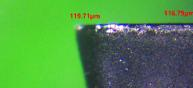
\includegraphics[width=0.3\linewidth]{tw-2.jpg} \\ \hline
	10 & 170.07 & 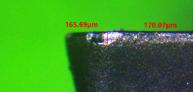
\includegraphics[width=0.3\linewidth]{tw-3.jpg} \\ \hline
	15 & 212.21 & 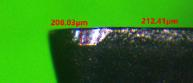
\includegraphics[width=0.3\linewidth]{tw-4.jpg} \\ \hline
	20 & 236.50 & 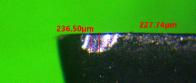
\includegraphics[width=0.3\linewidth]{tw-5.jpg} \\ \hline
	25 & 254.74 & 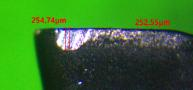
\includegraphics[width=0.3\linewidth]{tw-6.jpg} \\ \hline
	30 & 280.29 & 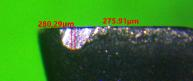
\includegraphics[width=0.3\linewidth]{tw-7.jpg} \\ \hline
	35 & 303.65 & 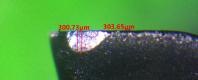
\includegraphics[width=0.3\linewidth]{tw-8.jpg} \\ \hline
	\end{tabular}
\end{table}

\end{appendices}

\clearpage
\newpage
\bibliography{references}

\end{document}